% -*- root: Dissertation.tex -*-
\documentclass[Dissertation.tex]{subfiles}
\graphicspath{{../Figures/}}
\begin{document}
\chapter{Robust DPG Methods for Transient Convection-Diffusion}
\label{sec:robust}
\section{Introduction}
The process of developing robust DPG methods for steady convection-diffusion was explored in \cite{DemkowiczHeuer,ChanHeuerThanhDemkowicz2012}.
In the sense, the main challenge is to come up with a correct test norm. The residual is measured
in the dual test norm, and the DPG method minimizes the residual. The residual can be interpreted
as a special {\em energy norm}. In other words, the DPG method delivers an orthogonal
projection in the energy norm. The task is especially challenging for singular perturbation
problems. Given a trial norm, we strive to determine a quasi-optimal test norm such that
the corresponding energy norm is robustly equivalent to the trial  norm of choice. An additional
difficulty comes from the fact that the optimal test functions should be easily approximated
with a simple enrichment strategy. For convection dominated diffusion, this means that
the test functions should not develop boundary layers. The task of determining the
quasi optimal test norm (we call it a {\em robust test norm} leads then to a stability analysis
for the adjoint equation which is the subject of this chapter. For a more general discussion
on the subject, see \cite{DPGEncyclopedia}.
In this chapter, two new robust norms are derived and numerical verifications of the theory are presented.

\section{Transient Convection-Diffusion}
In order to better illustrate choice of the $U$ and $V$ spaces, we introduce the transient convection-diffusion problem.
Consider spatial domain $\Omega$ and corresponding space-time domain $Q=\Omega\times[0,T]$ 
with boundary $\Gamma=\Gamma_-\cup\Gamma_+\cup\Gamma_0\cup\Gamma_T$ 
where $\Gamma_-$ is the inflow boundary ($\bfbeta\cdot\bfn_x<0$, where $\bfbeta$ is the convection vector and $\bfn_x$ is the outward spatial normal),
$\Gamma_+$ is the outflow boundary ($\bfbeta\cdot\bfn_x\geq0$), $\Gamma_0$ is the initial time boundary, 
and $\Gamma_T$ is the final time boundary. Let $\Gamma_h:=\bigcup\partial K$ denote the entire mesh skeleton, 
where $\partial K$ denotes the boundary of element $K$.
$\Gamma_{h_x}$ denotes any parts of the skeleton with a nonzero spatial normal and $\Gamma_{h_t}$ have a nonzero temporal normal.
% Given outward spatial normal $\bfn_x$ and convection vector $\bfbeta$, define inflow boundary $\Gamma_-\subset\Gamma_x$ where $\bfbeta\cdot\bfn_x<0$
% and outflow boundary $\Gamma_+$ where 

The transient convection-diffusion equation is
\begin{equation*}
\frac{\partial u}{\partial t}+\Div(\bfbeta u)-\epsilon\Delta u=f\,,
\end{equation*}
where $u$ is the quantity of interest, often interpreted to be a concentration of some quantity,
 % $\bfbeta$ is the convection vector,
$\epsilon$ is the  diffusion coefficient, and $f$ is the source term.

We apply flux boundary conditions on the inflow and trace boundary conditions on the outflow
\begin{align*}
\trace\LRp{\bfbeta\cdot u-\epsilon\Grad u}\cdot\bfn_x&=t_-\quad\text{on}\quad\Gamma_-\\
\trace\LRp{u}&=u_+\quad\text{on}\quad\Gamma_+\\
\trace\LRp{u}&=u_0\quad\text{on}\quad\Gamma_0\,.
\end{align*}
We note that Dirichlet boundary conditions also induce Dirichlet boundary conditions for the adjoint problem.  
Since the direction of convection is reversed for the adjoint convection-diffusion problem, 
this results in boundary layer adjoint solutions, which must be controlled using special weighted norms \cite{RoosStynesTobiska08,DemkowiczHeuer}.
% (cite Tobiska, Roos, Stynes, as well as Heuer/LD robustness paper #1).  
However, since the convection-diffusion operator is not self-adjoint, the Cauchy inflow boundary condition induces a Neumann boundary condition for the adjoint problem.  As a result, the adjoint solution does not contain boundary layers, simplifying the construction of a robust DPG method.

\subsection{Relevant Sobolev Spaces}
We begin by defining operators $\Gradxt u:=\vecttwo{\Grad u}{\pd{u}{t}}$ and $\Divxt\bfu:=\Div\bfu_x+\pd{u_t}{t}$, where $\bfu=(\bfu_x,u_t)$.
We will need the following Sobolev spaces defined on our space-time domain.
\begin{align*}
\HOneQ&=\LRc{u\in\LQ\,:\,\Grad u\in\LVecQ}\\
H^1_{xt}(Q)&=\LRc{u\in\LQ\,:\,\Gradxt u\in\LVecQ}\\
\bfH(\text{div},Q)&=\LRc{\bfsigma\in\LVecQ\,:\,\Div\bfsigma\in\LQ}\\
\bfH(\text{div}_{xt},Q)&=\LRc{\bfsigma\in\LVecQ\,:\,\Divxt\bfsigma\in\LQ}\\
\end{align*}
We will also need the corresponding broken Sobolev spaces.
\begin{align*}
H^1(Q_h)&=\LRc{u\in\LQ\,:\,u|_K\in\HOneK,\,K\in Q_h}&&=\prod_{K\in Q_h}H^1(K)\\
H^1_{xt}(Q_h)&=\LRc{u\in\LQ\,:\,u|_K\in H^1_{xt}(K),\,K\in Q_h}&&=\prod_{K\in Q_h}H^1_{xt}(K)\\
\bfH(\text{div},Q_h)&=\LRc{\bfsigma\in\LVecQ\,:\,u|_K\in\bfH(\text{div},K),\,K\in Q_h}&&=\prod_{K\in Q_h}\bfH(\text{div},K)\\
\bfH(\text{div}_{xt},Q_h)&=\LRc{\bfsigma\in\LVecQ\,:\,u|_K\in\bfH(\text{div}_{xt},K),\,K\in Q_h}&&=\prod_{K\in Q_h}\bfH(\text{div}_{xt},K)
\end{align*}
Consider the following trace operators:
\begin{align*}
\text{tr}^K_\text{grad} u&=u|_{\partial K_x} & u\in H^1(K)\\
\text{tr}^K_{\text{div}_{xt}} \bfsigma&=\bfsigma|_{\partial K_{xt}}\cdot\bfn_{K_{xt}} & \bfsigma\in \bfH(\text{div}_{xt},K)
\end{align*}
where $\partial K_x$ refers to spatial faces of element $K$, $\partial K_{xt}$ to the full space-time boundary, and $\bfn_{K_{xt}}$ is the unit outward normal on $\partial K_{xt}$.
The operators $\text{tr}_{grad}$ and $\text{tr}_{\text{div}_{xt}}$ perform the same operation element by element to produce the linear maps
\begin{align*}
\text{tr}_{\text{grad}}&\,:\,H^1(Q_h)\rightarrow\prod_{K\in Q_h}H^{1/2}(\partial K_x)\\
\text{tr}_{\text{div}_{xt}}&\,:\,\bfH(\text{div}_{xt},Q_h)\rightarrow\prod_{K\in Q_h}H^{-1/2}(\partial K_{xt})
\end{align*}
Finally, we define spaces of interface functions.
In order that our functions be single valued, we use the following definitions.
\begin{align*}
H^{1/2}(\Gamma_{h_x})&=\text{tr}_{\text{grad}}H^{1}(Q)\,,\\
H^{-1/2}_{xt}(\Gamma_h)&=\text{tr}_{\text{div}_{xt}}H(\text{div}_{xt},Q)\,.
\end{align*}
For more details on broken and trace Sobolev spaces, see \cite{BreakingSpaces}.

\subsection{Variational Formulations}
There are many possible manipulations that could be performed before arriving at a variational formulation. 
We begin by reformulating the problem in terms of the first order system:
\begin{equation}
\label{eq:confusionFirstOrder}
\begin{aligned}
\frac{1}{\epsilon}\bfsigma-\Grad u&=0\\
\Divxt\vecttwo{\bfbeta u-\bfsigma}{u}&=f\,.
\end{aligned}
\end{equation}
Multiplying \eqref{eq:confusionFirstOrder} by test functions $\bftau\in\LVecQ$ and $v\in\LQ$, we obtain the following 
``trivial'' variational formulation equivalent to the strong form:
\begin{equation}
\label{eq:confusionStrongBF}
	\begin{aligned}
		% u\in H^1_{xt}(Q)\,,\,\bfsigma\in\bfH(\text{div},Q)&\\
		&u\in H^1_{xt}(Q) &u&=u_+\quad &\text{on }\Gamma_+\\
		& &u&=u_0\quad &\text{on }\Gamma_0\\
		&\bfsigma\in \bfH(\text{div},Q)&(\bfbeta u-\epsilon\Grad u)\cdot\bfn&=t_-\quad &\text{on }\Gamma_-\\
		&\LRp{\frac{1}{\epsilon}\bfsigma,\bftau}-\LRp{\Grad u,\bftau}&&=0\quad&\forall\bftau\in\LVecQ\\
		&\LRp{\Divxt\vecttwo{\bfbeta u-\bfsigma}{u},v}&&=f\quad&\forall v\in\LQ\,.
	\end{aligned}
\end{equation}
% which is $L^2$-equivalent to the strong form.

We can now choose either to relax (integrate by parts and build in the boundary conditions) or strongly enforce each equation. 
The steady state case and resulting options are explored and analyzed in further detail in \cite{VariousVariational} 
and are termed the trivial formulation (don't relax anything), the classical formulation (relax the second equation), 
the mixed formulation (relax the first equation), and the ultra-weak formulation (relax both equations).
The stability constants for the four formulations are related, but the functional settings and norms of convergence change.
Early DPG work emphasized the ultra-weak formulation since in many ways it was the easiest to analyze, 
though recently the classical formulation has been under very active consideration.
In the interests of simpler analysis, we focus on the ultra-weak formulation in this chapter.
\begin{equation}
\label{eq:confusionUltraWeakBF}
	\begin{aligned}
		% &u\in L^2(Q) &u=g\quad &\text{on }\Gamma_+\\
		% &\bfsigma\in\LVecQ &(\bfbeta u-\epsilon\Grad u)\cdot\bfn=h\quad &\text{on }\Gamma_-\\
		&u\in L^2(Q)\,,\,\bfsigma\in\LVecQ\\
		&\LRp{\frac{1}{\epsilon}\bfsigma,\bftau}+\LRp{u,\Div\bftau}&=0\quad&\forall\bftau\in\bfH(\text{div},Q)\,:\,\bftau\cdot\bfn_x=0\text{ on }\Gamma_-\\
		&-\LRp{\vecttwo{\bfbeta u-\bfsigma}{u},\Gradxt v}&=f\quad&\forall v\in H^1_{xt}(Q)\,:\,v=0\text{ on }\Gamma_+\cup\Gamma_0\,,
	\end{aligned}
\end{equation}
We can remove the conditions on the test functions by introducing trace unknowns 
\begin{align*}
\hat u&=\trace(u)&\text{ on }\partial Q_x\\
\hat t&=\trace\vecttwo{\bfbeta u-\bfsigma}{u}\cdot\bfn_{xt}&\text{ on }\partial Q_{xt}\,.
\end{align*}
Our new ultra-weak formulation with conforming test functions is
\begin{equation}
\label{eq:confusionUltraWeakContinuousBF}
	\begin{aligned}
		&u\in L^2(Q)\,,\,\bfsigma\in\LVecQ\\
		&\hat u\in H^{1/2}(\partial Q_x)\,,\,&\hat u&=u_+&\text{ on }\Gamma_+\\
		&\hat t\in H^{-1/2}_{xt}(\partial Q)\,,\,&\hat t&=t_-&\text{ on }\Gamma_-\,,\quad\hat t=-u_0\text{ on }\Gamma_0\\
		&\LRp{\frac{1}{\epsilon}\bfsigma,\bftau}+\LRp{u,\Div\bftau}-\LRa{\hat u,\bftau\cdot\bfn_x}&&=0\quad&\forall\bftau\in\bfH(\text{div},Q)\\
		&-\LRp{\vecttwo{\bfbeta u-\bfsigma}{u},\Gradxt v}+\LRa{\hat t,v}&&=f\quad&\forall v\in H^1_{xt}(Q)\,.
	\end{aligned}
\end{equation}

\subsection{Broken Test Functions}
One of the key insights that led to the development of the DPG framework was the process of breaking test functions, 
that is testing with functions from larger broken Sobolev spaces, replacing $H^1_{xt}(Q)$ with  $H^1_{xt}(Q_h)$ 
and $\bfH(\text{div},Q)$ with $\bfH(\text{div},Q_h)$.
Discretizing such spaces is much simpler than standard spaces which require enforcement of global continuity conditions.
The cost of introducing broken spaces is that we have to extend our interface unknowns $\hat u$ and $\hat t$ 
to live on the mesh skeleton. % $\Gamma_h=\bigcup_{K\in Q_h}\partial K$.
Our ultra-weak formulation with broken test functions looks like
\begin{equation}
\label{eq:confusionUltraWeakBrokenBF}
	\begin{aligned}
		&u\in L^2(Q)\,,\,\bfsigma\in\LVecQ\\
		&\hat u\in H^{1/2}(\Gamma_{h_x})\,,\,&\hat u&=u_+&\text{ on }\Gamma_+\\
		&\hat t\in H^{-1/2}_{xt}(\Gamma_h)\,,\,&\hat t&=t_-&\text{ on }\Gamma_-\,,\quad\hat t=-u_0\text{ on }\Gamma_0\\
		&\LRp{\frac{1}{\epsilon}\bfsigma,\bftau}+\LRp{u,\Div\bftau}-\LRa{\hat u,\bftau\cdot\bfn_x}&&=0\quad&\forall\bftau\in\bfH(\text{div},Q_h)\\
		&-\LRp{\vecttwo{\bfbeta u-\bfsigma}{u},\Gradxt v}+\LRa{\hat t,v}&&=f\quad&\forall v\in H^1_{xt}(Q_h)\,.
	\end{aligned}
\end{equation}
The main consequence of breaking test functions is that it reduces the cost of solving for optimal test functions from a global solve 
to an embarrassingly parallel solve element-by-element.
Now that we've derived a suitable variational formulation, we are left with the task of selecting a test norm with which to compute our optimal test functions.
% Moro \etal \cite{MoroNguyenPeraire11} handle the flux unknowns with a numerical flux in the hybridized DPG (HDPG) method, but the standard DPG method treats
% these as new unknowns to be solved for.
% We still haven't specified our trial space $U$, but the rule is that for every integration by parts, a new skeleton unknown is introduced.
% Most DPG considerations have used the ultra-weak variational formulation and break a second order PDE into 
% a system of first order PDEs. 
% This introduces a trace unknown (through the constitutive law) and a flux unknown (through the conservation law) with field variables that live in $L^2$.
% It is actually possible to create a DPG method for any well-posed variational formulation, including the classical one \cite{PrimalDPG}.
% But Demkowicz and Gopalakrishnan also formulated 
% a \emph{primal DPG} method \cite{PrimalDPG} for second order equations that does not introduce a trace unknown.
% The overall number of interface unknowns in the primal DPG method is the same, however, since the solution is required to be $H^1$ conforming 
% and the trace unknowns are essentially hidden there.

\section{Robust Test Norms}
The final unresolved choice is what norm to apply to the $V$ space.
This is one of the most important factors in designing a robust DPG method as the corresponding Riesz operator 
needs to be inverted to solve for the optimal test functions.
If the norm produces unresolved boundary layers in the auxiliary problem, then many of the attractive features of DPG may fall apart.
This is the primary emphasis of this chapter.
The problem of constructing stable test norms for steady convection-diffusion was addressed in \cite{DemkowiczHeuer,ChanHeuerThanhDemkowicz2012}.
In this chapter, we extend that work to transient convection-diffusion in space-time.

% Talk about robustness assuming infinite dimensional V
We define a robust test norm such that the $L^2$ norm of the solution 
is bounded by the energy norm of the solution with a constant independent of $\epsilon$.
We can rewrite any ultra-weak formulation with broken test functions as the following
bilinear form with group variables:
\[
b\LRp{\LRp{u,\hat u},v} = \LRp{u,A^* v}_{L^2} + \LRa{\uh, \jump{v}}_{\Gh}
\]
where $A^*$ represents the adjoint.
In the case of convection-diffusion, $u:=\LRc{u,\bfsigma}$, $\hat u:=\LRc{\hat u,\hat t}$, $v:=\LRc{v,\bftau}$.

Note that for conforming $v^*$ satisfying $A^* v^* = u$
\begin{align*}
&\norm{u}_{L^2}^2= b(u,v^*)
=\frac{b(u,v^*)}{\norm{v^*}_V} \norm{v^*}_V\\
&\quad\leq\sup_{v^*\neq0}\frac{|b(u,v^*)|}{\norm{v^*}}\norm{v^*}
=\norm{u}_E \norm{v^*}_V\,.
\end{align*}
This defines a necessary condition for robustness, namely that
\begin{align}
\label{eq:necessaryCondition}
\norm{v^*}_V\lesssim\norm{u}_{L^2}\,.
\end{align}
If this condition is satisfied, then we get our final result:
\begin{align*}
\norm{u}_{L^2}\lesssim\norm{u}_E\,.
\end{align*}

So far, we've assumed that our finite set of optimal test functions are assembled from an infinite dimensional space.
In practice, we have found it to be sufficient to use an ``enriched'' space of higher
polynomial dimension than the trial space \cite{PracticalDPG}.
This adds an additional requirement when assembling a robust test norm, namely that our optimal test functions should be adequately representable within this enriched space.
We illustrate this point by considering three norms which satisfy the above conditions for 1D steady convection-diffusion.
The graph norm is $\LRp{\norm{A^*v}_{L^2}^2+\norm{v}_{L^2}^2}^{\frac{1}{2}}$:
\begin{equation*}
\norm{(v,\bftau)}^2=
\norm{\Div\bftau-\bfbeta\cdot\Grad v}^2
+\norm{\frac{1}{\epsilon}\bftau+\Grad v}^2
+\norm{v}^2
+\norm{\bftau}^2\,.
\end{equation*}
\begin{remark}
In the DPG technology, the test norm must be {\em localizable}, i.e.,
$$
\Vert v \Vert^2_{V} = \sum_{K} \Vert v \Vert^2_{V(K)}
$$
where $\Vert v \Vert_{V(K)}$ denotes a test norm (and not just a seminorm) for the
element test space. In practice this means the addition of properly scaled $L^2$-terms.
Without those terms, we could not invert the Riesz operator on the element level.
Addition of the $L^2$ terms does not necessarily contradict the robustness of the norm,
see the discussion in \cite{DPGEncyclopedia} on bounded below operators. An alternate
strategy has been explored in \cite{EllisLC} where we enforce element conservation
property 
by securing the presence of a constant function in the element test space. The residual
is then minimized only over the orthogonal complement to the constants which eliminates
the need for adding the $L^2$-term to the test norm.
\end{remark}
The robust norm was derived in \cite{ChanHeuerThanhDemkowicz2012}:
\begin{align*}
\norm{(v,\bftau)}^2&=
\norm{\bfbeta\cdot\Grad v}^2
+\epsilon\norm{\Grad v}^2
+\min\LRp{\frac{\epsilon}{h^2},1}\norm{v}^2
\\&\quad
+\norm{\Div\bftau}^2
+\min\LRp{\frac{1}{h^2},\frac{1}{\epsilon}}\norm{\bftau}^2\,.
\end{align*}
The case for the coupled robust norm was made in \cite{JesseDissertation}:
\begin{align*}
\norm{(v,\bftau)}^2&=
\norm{\bfbeta\cdot\Grad v}^2
+\epsilon\norm{\Grad v}^2
+\min\LRp{\frac{\epsilon}{h^2},1}\norm{v}^2
\\&\quad
+\norm{\Div\bftau-\bfbeta\cdot\Grad v}^2
+\min\LRp{\frac{1}{h^2},\frac{1}{\epsilon}}\norm{\bftau}^2\,.
\end{align*}
The argument for the coupled norm was that in certain cases we noticed pollution of $u$ from errors in $\bfsigma$,
for example at singularities in $\bfsigma$, $u$ also exhibited degraded quality with the robust norm. 
The coupled robust norm seemed to relax this behavior, i.e. errors in $u$ appear more independent of errors in $\bfsigma$.

The bilinear form and test norm define a mapping from input trial functions to an optimal test function:
\[
T=R_V^{-1}B\,:\,U\rightarrow V\,.
\]
Below, we plot the optimal test functions produced given $\epsilon=10^{-2}, $a representative trial function $u=x-\frac{1}{2}$,
and either the graph norm, the robust norm, or the coupled robust norm.
Note that the optimal test functions will be different for any other trial function.
In the left column, we see the fully resolved \emph{ideal} optimal test function that DPG theory relies on.
On the right, we see the approximated optimal test function using a enriched cubic test space.
\begin{figure}[ht]
\centering
\begin{subfigure}[t]{0.45\textwidth}
\centering
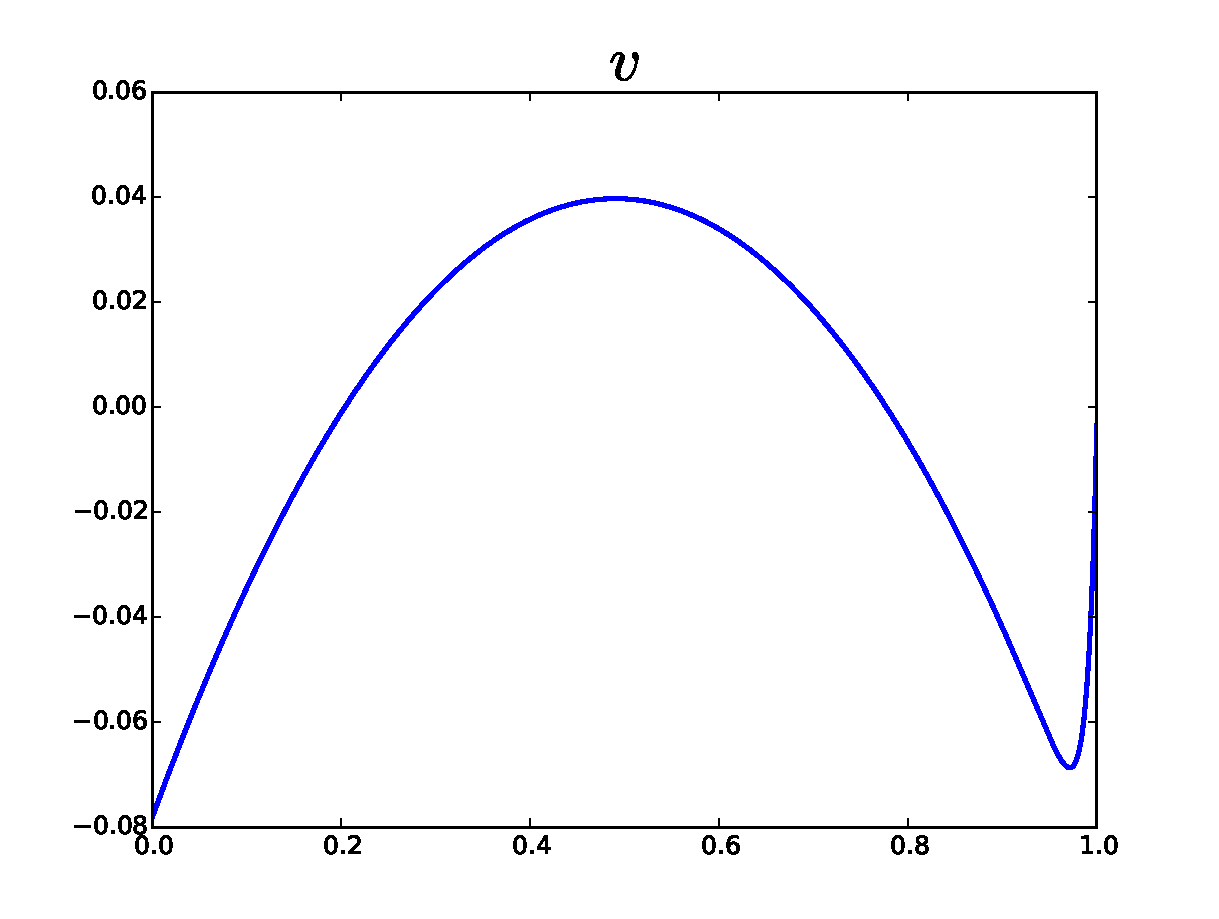
\includegraphics[width=\textwidth]{OptimalTestFunctions/uLinear_1e-2/steady/graph_steady_v}\\
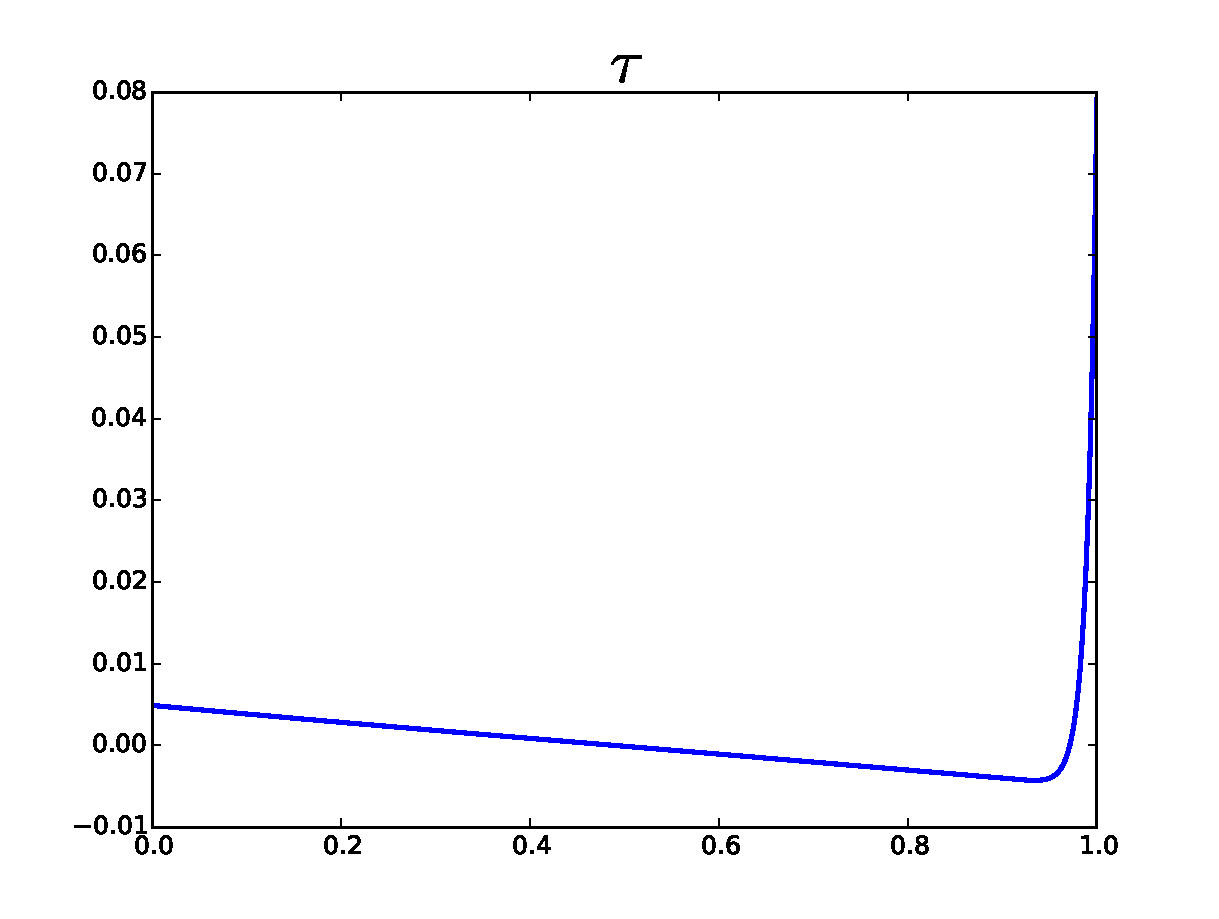
\includegraphics[width=\textwidth]{OptimalTestFunctions/uLinear_1e-2/steady/graph_steady_tau}\\
\caption{Ideal}
\label{fig:idealGraph}
\end{subfigure}
\begin{subfigure}[t]{0.45\textwidth}
\centering
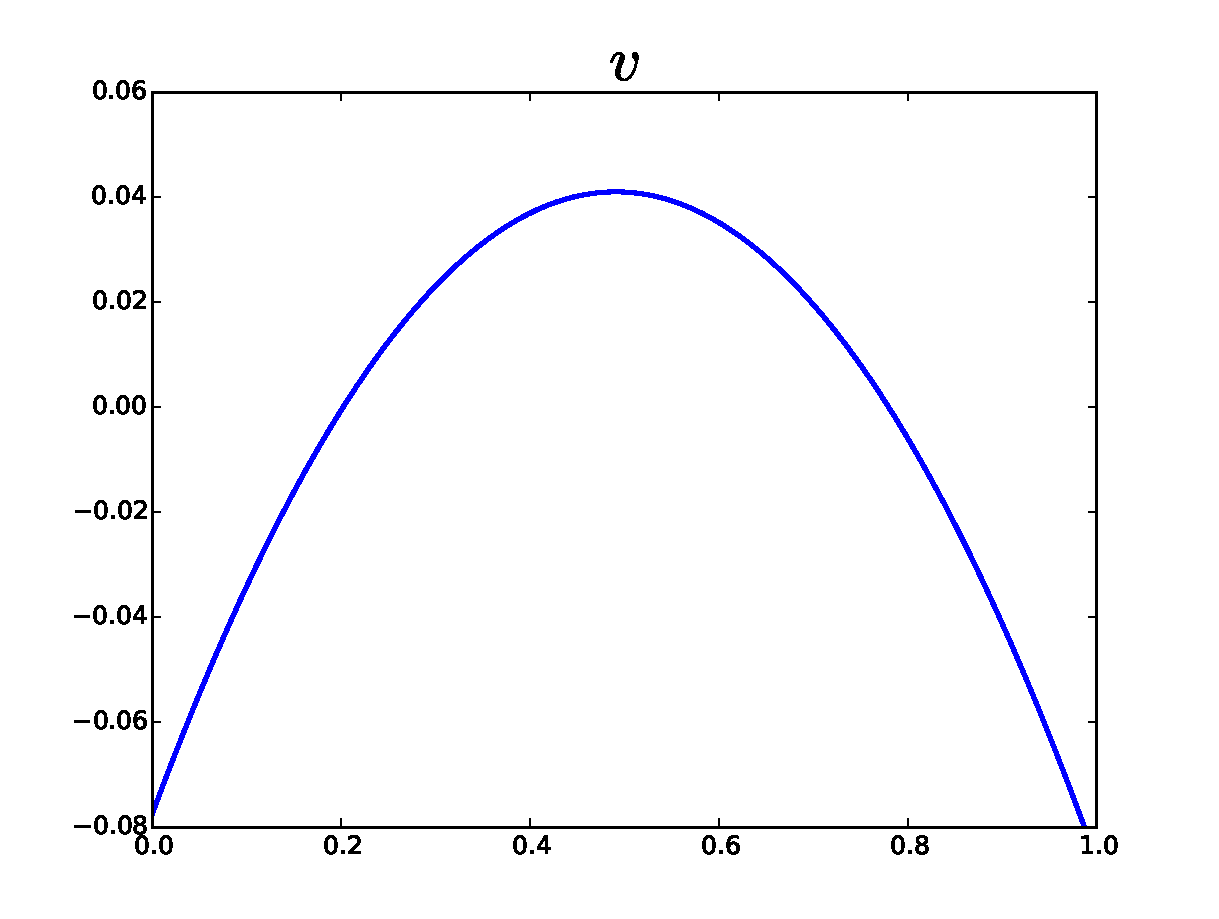
\includegraphics[width=\textwidth]{OptimalTestFunctions/uLinear_1e-2/steady/graph_steady_v_approx3}\\
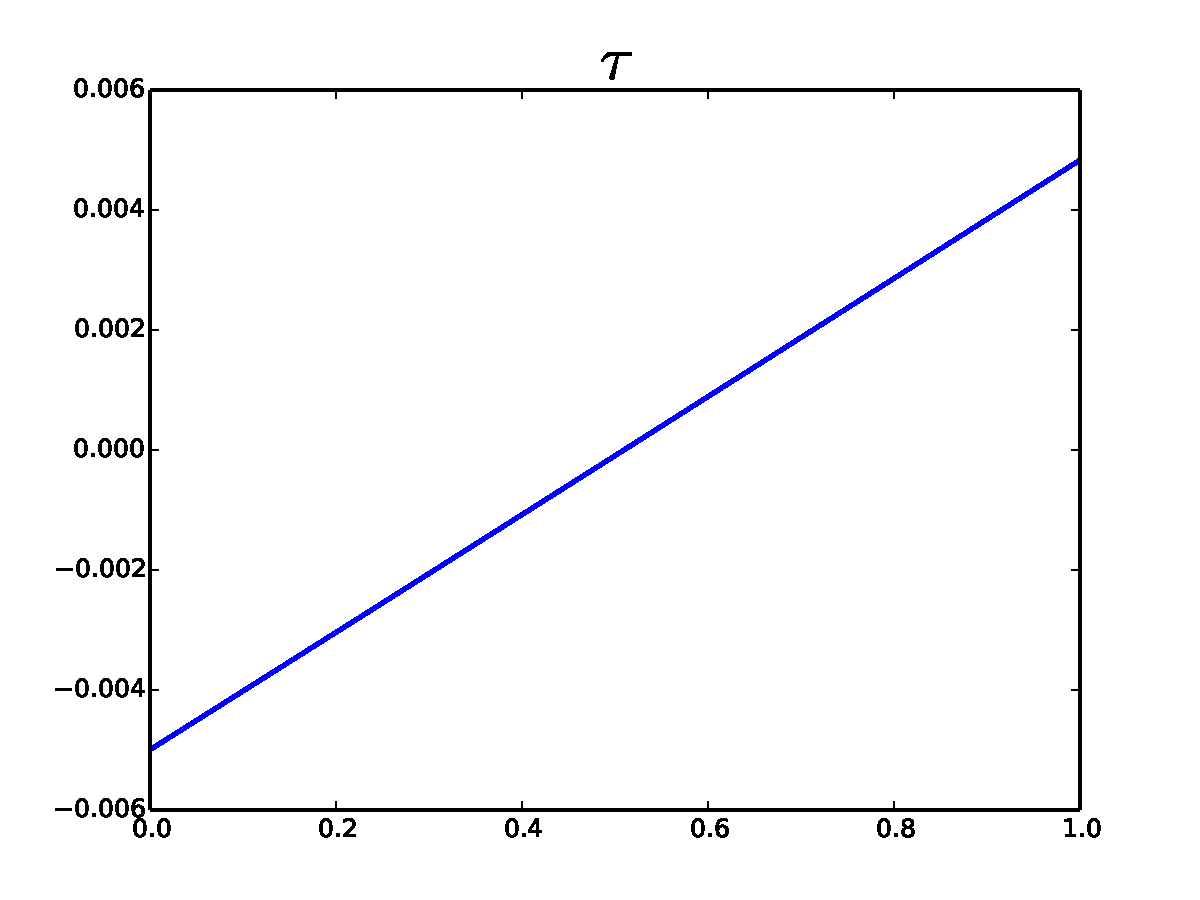
\includegraphics[width=\textwidth]{OptimalTestFunctions/uLinear_1e-2/steady/graph_steady_tau_approx3}\\
\caption{Approximated}
\label{fig:approxGraph}
\end{subfigure}
\caption{Graph norm optimal test functions for $u=x-\frac{1}{2}$}
\label{fig:optimalGraph}
\end{figure}

\begin{figure}[ht]
\centering
\begin{subfigure}[t]{0.45\textwidth}
\centering
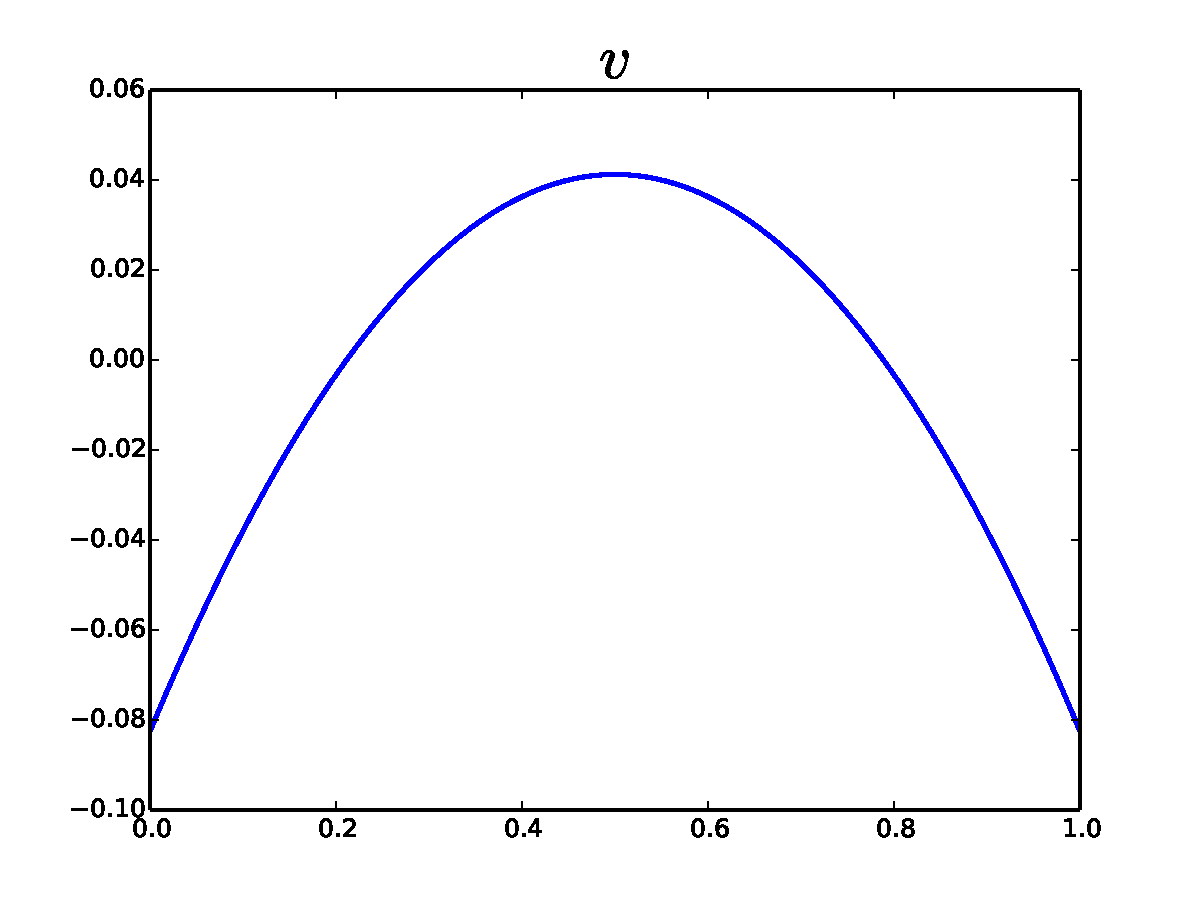
\includegraphics[width=\textwidth]{OptimalTestFunctions/uLinear_1e-2/steady/robust_steady_v}\\
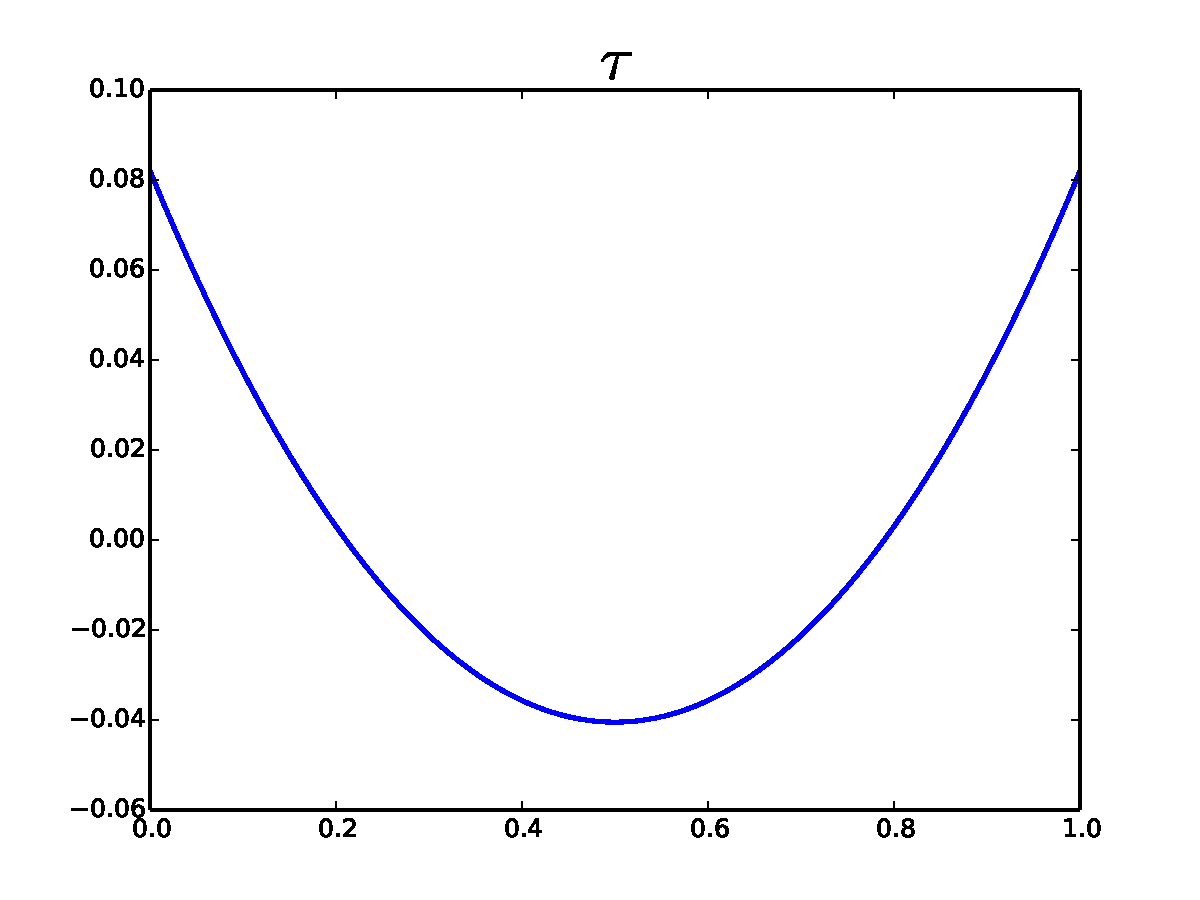
\includegraphics[width=\textwidth]{OptimalTestFunctions/uLinear_1e-2/steady/robust_steady_tau}\\
\caption{Ideal}
\label{fig:idealRobust}
\end{subfigure}
\begin{subfigure}[t]{0.45\textwidth}
\centering
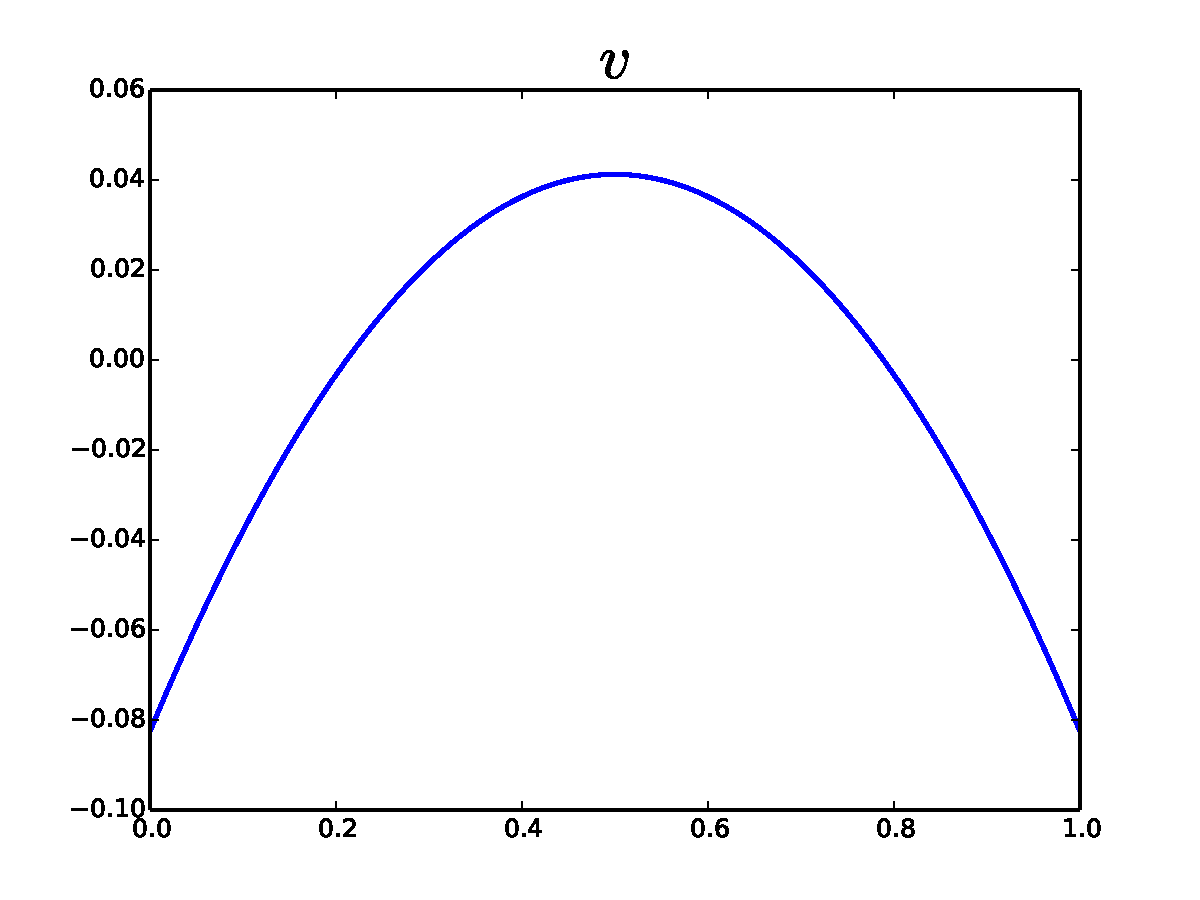
\includegraphics[width=\textwidth]{OptimalTestFunctions/uLinear_1e-2/steady/robust_steady_v_approx3}\\
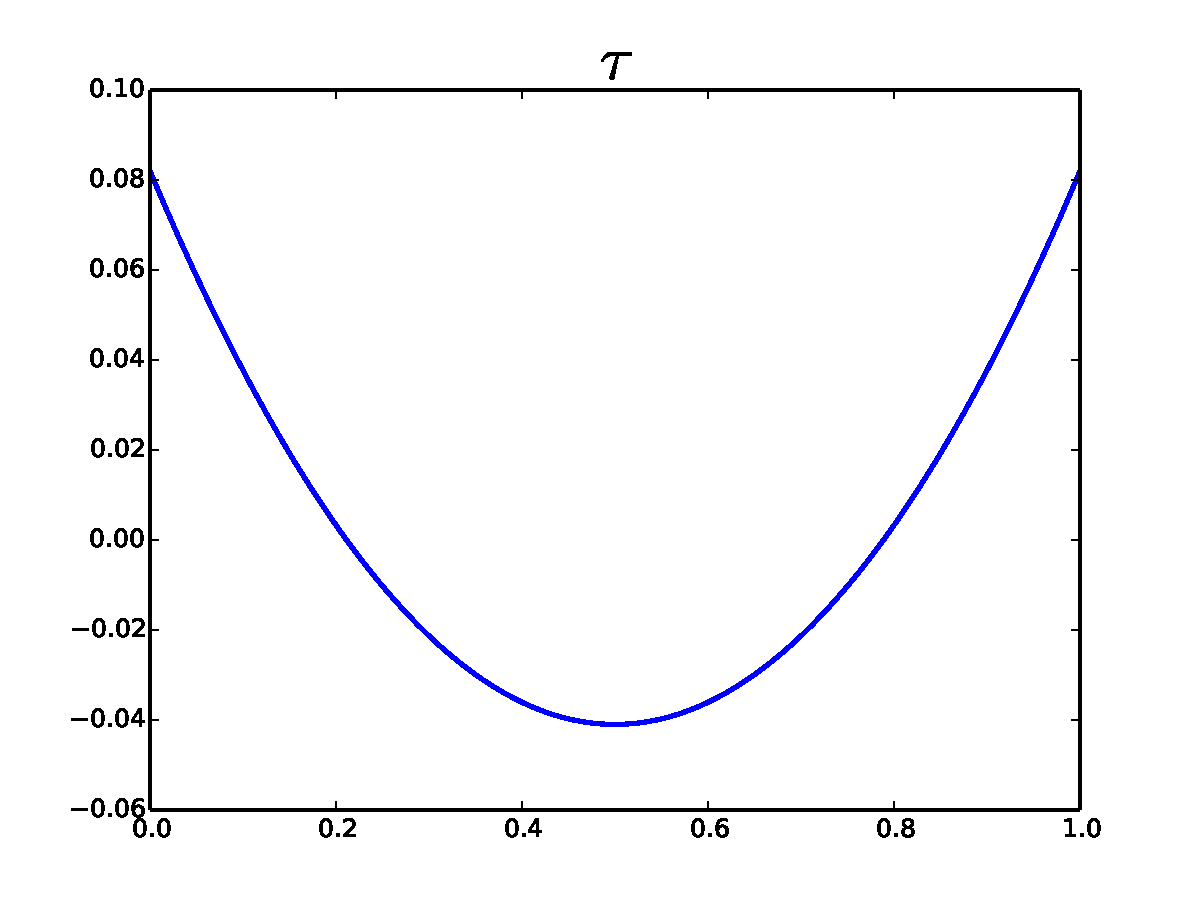
\includegraphics[width=\textwidth]{OptimalTestFunctions/uLinear_1e-2/steady/robust_steady_tau_approx3}\\
\caption{Approximated}
\label{fig:approxRobust}
\end{subfigure}
\caption{Robust norm optimal test functions for $u=x-\frac{1}{2}$}
\label{fig:optimalRobust}
\end{figure}

\begin{figure}[ht]
\centering
\begin{subfigure}[t]{0.45\textwidth}
\centering
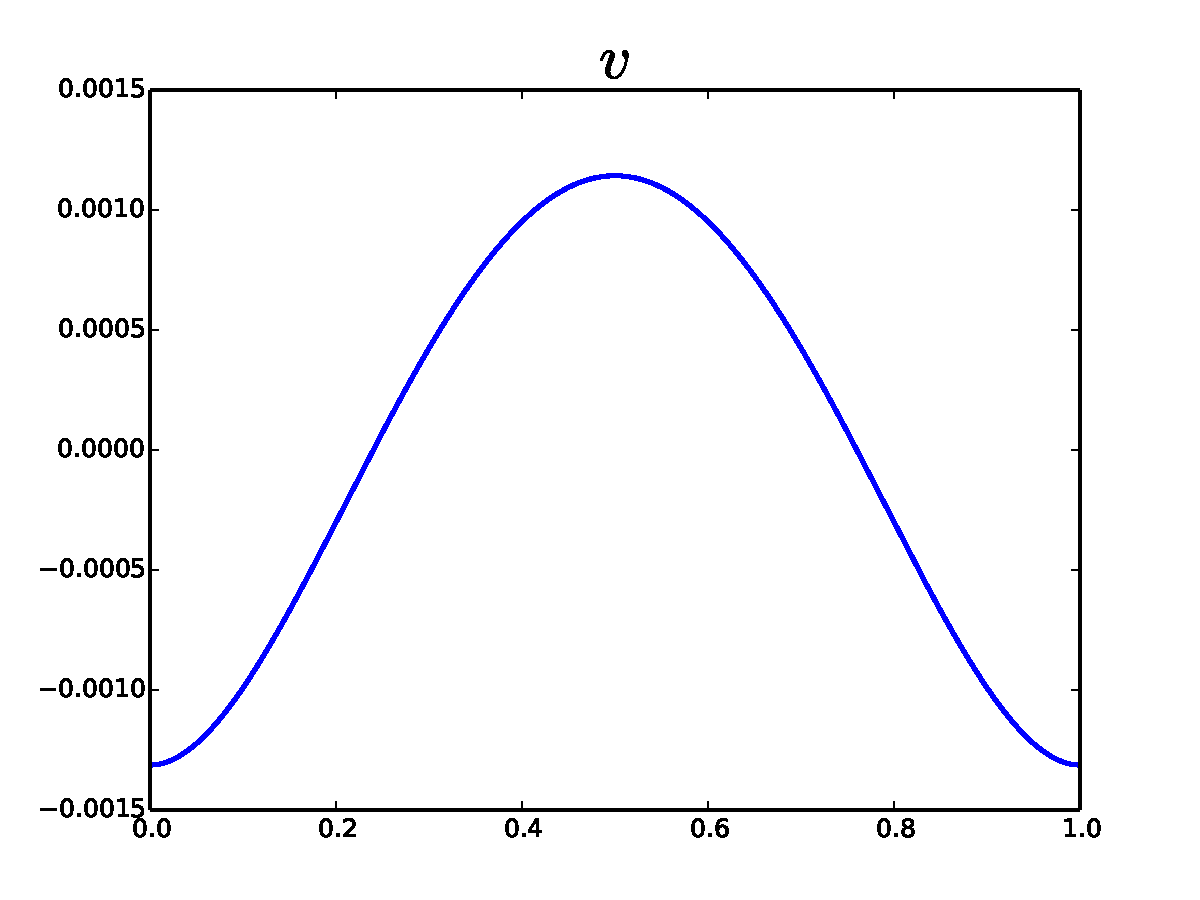
\includegraphics[width=\textwidth]{OptimalTestFunctions/uLinear_1e-2/steady/coupledrobust_steady_v}\\
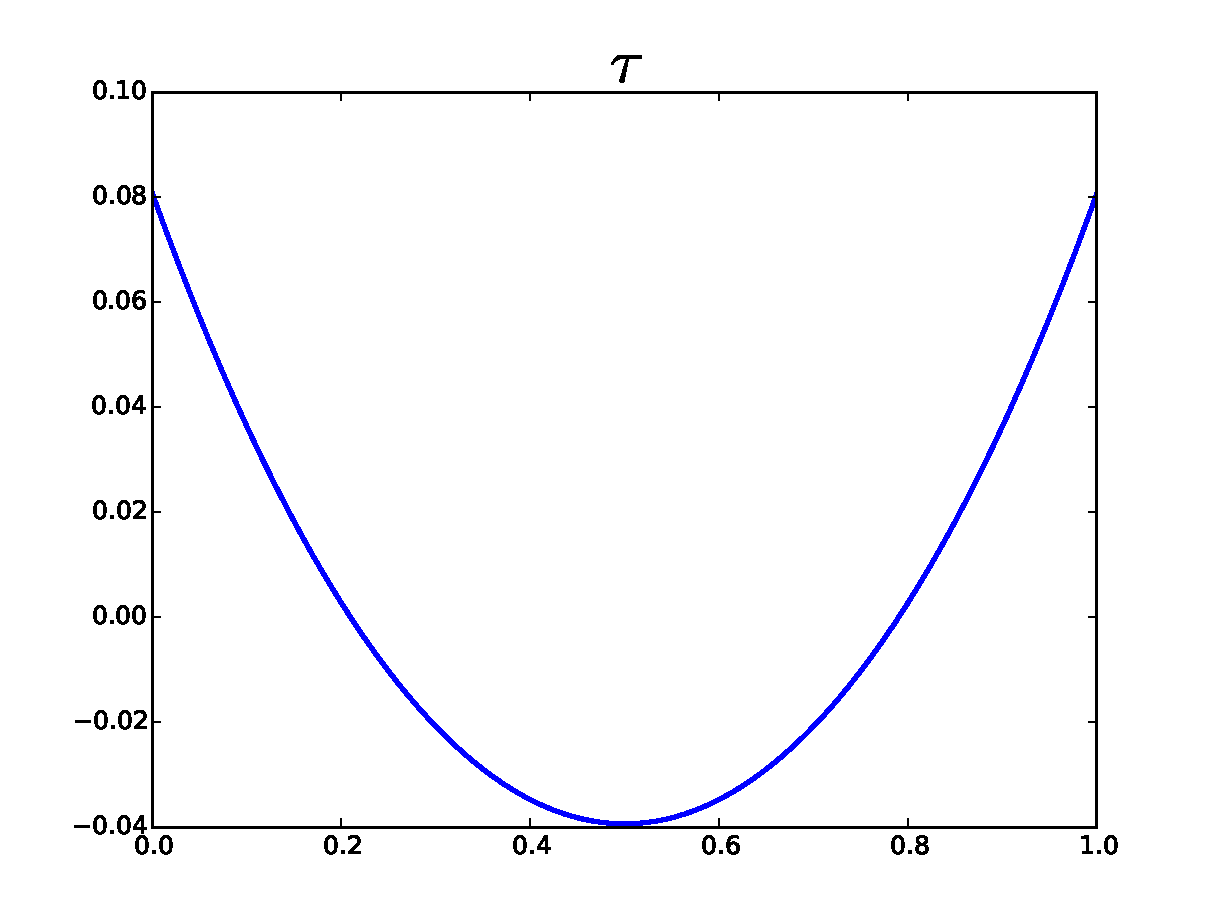
\includegraphics[width=\textwidth]{OptimalTestFunctions/uLinear_1e-2/steady/coupledrobust_steady_tau}\\
\caption{Ideal}
\label{fig:idealCoupledRobust}
\end{subfigure}
\begin{subfigure}[t]{0.45\textwidth}
\centering
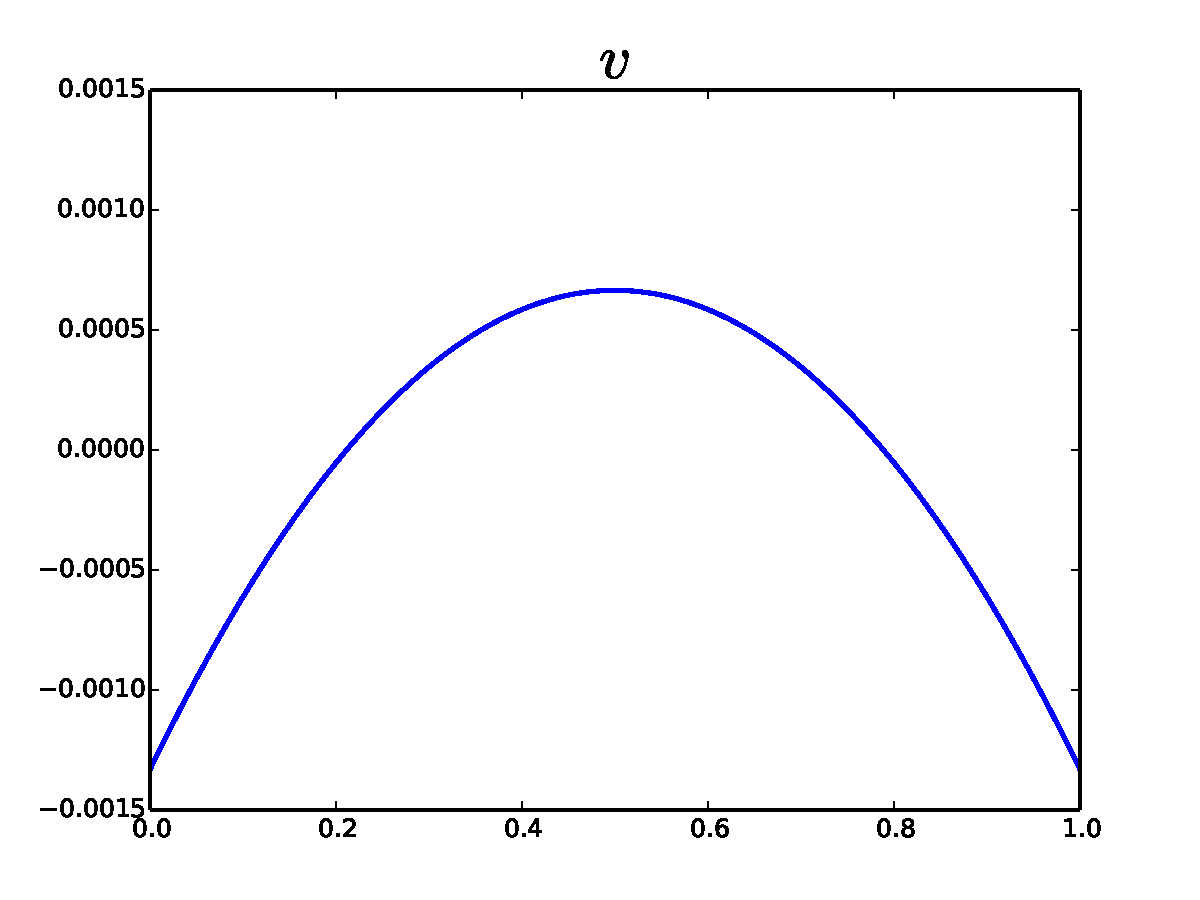
\includegraphics[width=\textwidth]{OptimalTestFunctions/uLinear_1e-2/steady/coupledrobust_steady_v_approx3}\\
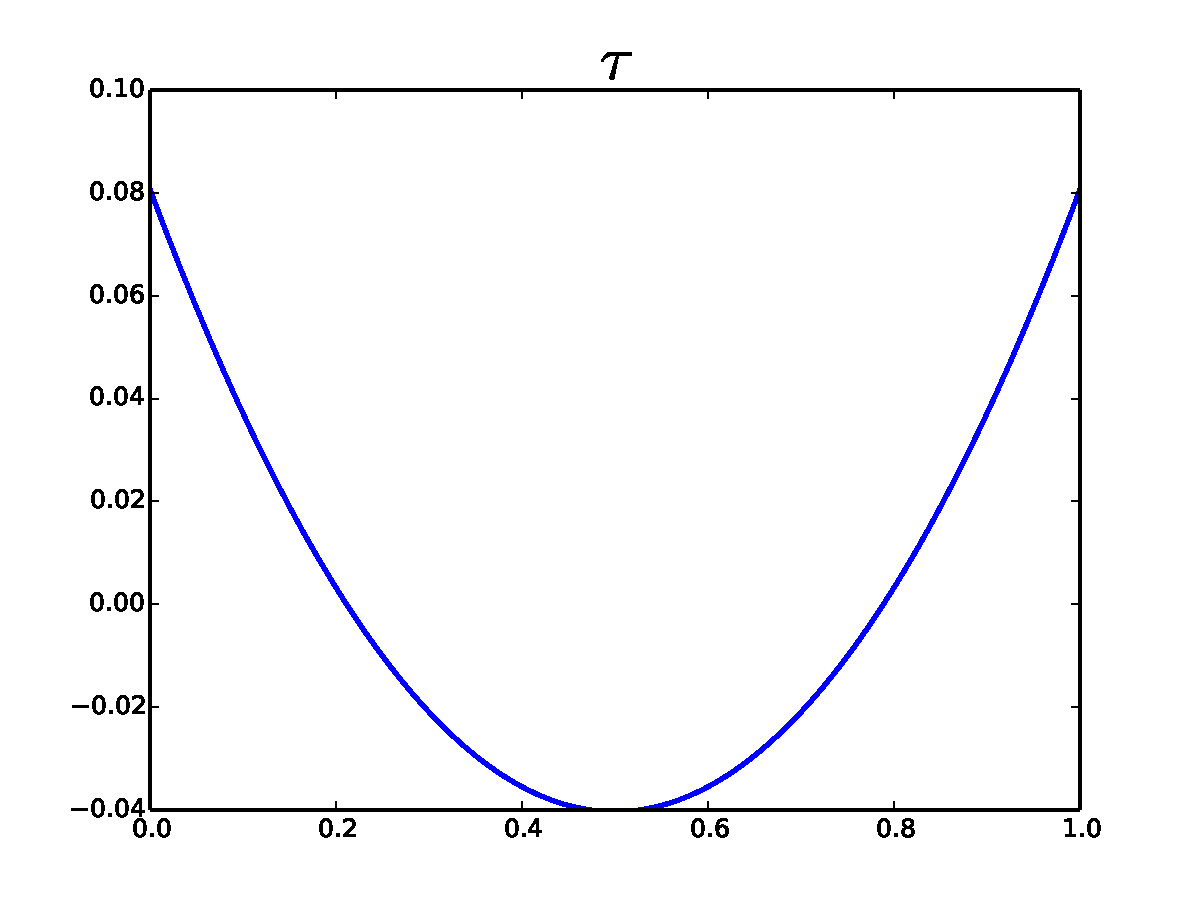
\includegraphics[width=\textwidth]{OptimalTestFunctions/uLinear_1e-2/steady/coupledrobust_steady_tau_approx3}\\
\caption{Approximated}
\label{fig:approxCoupledRobust}
\end{subfigure}
\caption{Coupled robust norm optimal test functions for $u=x-\frac{1}{2}$}
\label{fig:optimalCoupledRobust}
\end{figure}

Mathematically, the graph norm satisfies the necessary condition to be a robust norm, but the ideal optimal test functions contain strong boundary
layers which can not be realistically approximated with the provided enriched space.
If the approximated optimal test functions can not come sufficiently close to the ideal, then the whole DPG theory falls apart.
See \cite{PracticalDPG} for more discussion.
This provides an additional condition on a test norm before we can truly call it robust: the ideal test functions must be adequately representable within 
the provided enriched space.
This ultimately comes down to an analysis of the relative magnitudes of individual terms within the test norm, usually attempting to bound reactive or convective terms by diffusive terms.
The coupled robust norm satisfies condition \eqref{eq:necessaryCondition} and also produces relatively smooth optimal test functions that can be sufficiently approximated
with a cubic polynomial space.
Niemi \etal attempted to approximate boundary layers in optimal shape functions with Shishkin meshes \cite{NiemiShishkin,niemi2013discontinuous}.

\subsection{Application to Transient Convection-Diffusion}
Now we present the analysis leading to two robust norms for transient convection-diffusion.
Consider the problem with homogeneous boundary conditions
\begin{align*}
\frac{1}{\epsilon}\bfsigma-\Grad u &=0\\
\pd{u}{t} + \bfbeta\cdot\Grad u - \Div\bfsigma &= f\\
\beta_n u-\epsilon\pd{u}{n} &= 0 \text{ on } \Gamma_-\\
u &= 0 \text{ on } \Gamma_+\\
u &= u_0 \text{ on } \Gamma_0.
\end{align*}
% where $\Div\bfbeta=0$ and $\norm{\Grad\bfbeta}_{L^\infty}\le C_{\bfbeta}$.
Let $\tilde\bfbeta:=\vecttwo{\bfbeta}{1}$, then we can rewrite this as
\begin{align*}
\frac{1}{\epsilon}\bfsigma-\Grad u &=0\\
\tilde\bfbeta\cdot\Gradxt u - \Div\bfsigma &= f\\
% \Divxt\vecttwo{\bfbeta u-\bfsigma}{u}&=f\\
\beta_n u-\epsilon\pd{u}{n} &= 0 \text{ on } \Gamma_-\\
u &= 0 \text{ on } \Gamma_+\\
u &= u_0 \text{ on } \Gamma_0.
\end{align*}
The adjoint operator $A^*$ is given by 
\[
A^*(v,\bftau)=\LRp{\frac{1}{\epsilon}\bftau+\Grad v,-\tilde\bfbeta\cdot\Gradxt v+\Div\bftau}\,.
\]
We decompose now the continuous adjoint problem
\[
A^*(v,\bftau)=(\bff,g)
\]
into two cases
% We load the adjoint problem with:
% a discontinuous part
% \textcolor{red}{(Dr. Demkowicz, what kind of argument do we want to use to avoid dealing with this part? I assume it's something to do with breaking test functions.)}
% \begin{align*}
% \frac{1}{\epsilon}\bftau_0+\Grad v_0 &=0\\
% -\tilde\bfbeta\cdot\Gradxt v_0 + \Div\bftau_0 &= 0\\
% \bftau_0\cdot\bfn_x &= \bftau\cdot\bfn_x \text{ on } \Gamma_-\cup\Gamma_0\\
% v_0 &= v \text{ on } \Gamma_+\\
% v_0 &= v \text{ on } \Gamma_T\\
% \jump{v_0}&=\jump{v} \text{ on } \Gamma_h^0\\
% \jump{\bftau_0\cdot\bfn_x}&=\jump{\bftau_0\cdot\bfn_x} \text{ on } \Gamma_{hx}^0\,,
% \end{align*}
a continuous part with forcing term $g$
\begin{align*}
\frac{1}{\epsilon}\bftau_1+\Grad v_1 &=0\\
-\tilde\bfbeta\cdot\Gradxt v_1 + \Div\bftau_1 &= g\\
\bftau_1\cdot\bfn_x &= 0 \text{ on } \Gamma_-\\
v_1 &= 0 \text{ on } \Gamma_+\\
v_1 &= 0 \text{ on } \Gamma_T\,,
\end{align*}
and a continuous part with forcing $\bff$
\begin{align*}
\frac{1}{\epsilon}\bftau_2+\Grad v_2 &=\bff\\
-\tilde\bfbeta\cdot\Gradxt v_2 + \Div\bftau_2 &= 0\\
\bftau_2\cdot\bfn_x &= 0 \text{ on } \Gamma_-\\
v_2 &= 0 \text{ on } \Gamma_+\\
v_2 &= 0 \text{ on } \Gamma_T\,.
\end{align*}
(The boundary conditions can be derived by taking the ultra-weak formulation and choosing boundary conditions such that the temporal flux and spatial flux terms $\LRa{\uh, \jump{\tau_n}}_{\Gamma_{out}}$ and $\LRa{\hat t_n,\jump{v}}_{\Gamma_{in}}$ are zero.)

We can then derive that the test norms
\begin{align}
\label{eq:robustnorm}
\norm{\LRp{v,\bftau}}_{V,K}^2 &\coloneqq
\norm{\tilde\bfbeta\cdot\Gradxt v}_K^2
+ \epsilon\norm{\Grad v}_K^2
+ \norm{v}^2_K\\\nonumber&\quad
+ \norm{\Div \bftau}_K^2
+ \frac{1}{\epsilon}\norm{\bftau}_K^2\,,
\end{align}
and
\begin{align}
\label{eq:coupledrobustnorm}
\norm{\LRp{v,\bftau}}_{V,K}^2 &\coloneqq
\norm{\tilde\bfbeta\cdot\Gradxt v}_K^2
+ \epsilon\norm{\Grad v}_K^2
+ \norm{v}^2_K\\\nonumber&\quad
+ \norm{\Div \bftau - \tilde\bfbeta\cdot\Gradxt v}_K^2
+ \frac{1}{\epsilon}\norm{\bftau}_K^2\,,
\end{align}
respectively designated the \emph{robust} test norm and the \emph{coupled robust} test norm,
provide the necessary bound $\norm{v^*}_V \lesssim \norm{u}_{\LQ}$.
\begin{remark}
We haven't developed a mathematical theory for it, but we've also had numerical success with a norm that 
we've dubbed the NSDecoupled norm because we first stumbled on it during experiments with compressible
Navier-Stokes:
\begin{align*}
\norm{\LRp{v,\bftau}}_{V,K}^2 &\coloneqq
\norm{\bfbeta\cdot\Grad v+\pd{v}{t}}_K^2
+ \norm{\Grad v}_K^2
+ \norm{v}^2_K
\\\nonumber&\quad
+ \norm{\Div \bftau}_K^2
+ \frac{1}{h^2}\norm{\bftau}_K^2\,.
\end{align*}
We mention it because it appeared to be the most successful in simulations
of the moving piston problem in \ref{sec:piston}.
\end{remark}

In the following lemmas we establish the following bounds:
\begin{itemize}
\item Bound on $\norm{\LRp{v_1,\bftau_1}}_V$. 
Lemma~\ref{lem:convective} gives $\norm{\tilde\bfbeta\cdot\Gradxt v_1}\leq\norm{g}$.
Since $\Div\bftau_1=g+\tilde\bfbeta\cdot\Gradxt v_1$, 
\[
\norm{\Div\bftau_1}\leq\norm{g}+\norm{\tilde\bfbeta\cdot\Gradxt v_1}\leq 2\norm{g}.
\]
Or, the fact that $\Div\bftau-\tilde\bfbeta\cdot\Gradxt v_1=g$ clearly gives
\[
\norm{\Div \bftau - \tilde\bfbeta\cdot\Gradxt v_1}=\norm{g}.
\]
% Also, clearly
% \[
% \norm{\bfbeta\cdot\Grad v_1}\leq\norm{\tilde\bfbeta\cdot\Gradxt v_1}\leq\norm{g}.
% \]
Lemma~\ref{lem:l2} gives $\norm{v_1}^2+\epsilon\norm{\Grad v_1}^2\leq\norm{g}^2$.
Since $\epsilon^{1/2}\Grad v_1=-\epsilon^{-1/2}\bftau_1$,
\[
\frac{1}{\epsilon}\norm{\bftau_1}^2\leq\norm{g}^2.
\]
Thus, all $(v_1,\bftau_1)$ terms in \eqref{eq:robustnorm} and \eqref{eq:coupledrobustnorm} are accounted for, 
guaranteeing at least robust control of $u$.
\item Bound on $\norm{\LRp{v_2,\bftau_2}}_V$. 
The fact that $\Div\bftau-\tilde\bfbeta\cdot\Gradxt v=0$ clearly gives
\[
\norm{\Div \bftau - \tilde\bfbeta\cdot\Gradxt v_2}=0\leq\norm{\bff}.
\]
Lemma~\ref{lem:l2} gives $\norm{v_2}^2+\epsilon\norm{\Grad v_2}^2\leq\epsilon\norm{\bff}^2$.
Since $\epsilon^{1/2}\Grad v_2=\bff-\epsilon^{-1/2}\bftau_2$,
\[
\frac{1}{\epsilon}\norm{\bftau_2}^2\leq(1+\epsilon)\norm{\bff}^2.
\]
We have not been able to develop bounds on $\norm{\tilde\bfbeta\cdot\Gradxt v_2}$ and $\norm{\Div\bftau}$ 
which means that we can not guarantee robust control of $\bfsigma$ with with provided test norms.
% Intuitively since $\bfsigma$ is a spatial variable, it may not make sense to speak of controlling it 
% Finally,
% \[
% \norm{\bfbeta\cdot\Grad v_2}\leq\norm{\bfbeta}_\infty\norm{\Grad v_2}\leq\norm{\bfbeta}_\infty\norm{\bff}.
% \]
% Thus, all $(v_2,\bftau_2)$ terms in \eqref{eq:robustnorm} are accounted for.
\end{itemize}

We proceed now with the technical estimates.
% Our goal is to analyze the stability properties of the adjoint equations by deriving bounds of the form
% $\norm{(v_1,\bftau_1)}_V\leq\norm{g}_\LQ$ and $\norm{(v_2,\bftau_2)}_V\leq\norm{f}_\LQ$.

% \textcolor{red}{Insert conditions on $\bfbeta$}
\begin{lemma}
\label{lem:l2}
For the duration of this lemma, let $v:=v_1+v_2$.
Assuming the advection field $\bfbeta$ is incompressible, i.e. $\Div\bfbeta=0$,
\[
\norm{v}^2+\epsilon\norm{\Grad v}^2\leq\norm{g}^2+\epsilon\norm{\bff}^2\,.
\]
\end{lemma}
\begin{proof}
Define $w=e^{t}v$ and note that $\pd{w}{t}=\LRp{\pd{v}{t}+v}e^{t}$ while
all spatial derivatives go through.
%  $\Grad w=\cancelto{0}{\Grad e^{t}} v+e^{t}\Grad v$ and
% $\Div(\bfbeta w)=\Div(\bfbeta)e^{t} v+\bfbeta\cdot e^{t}\Grad v$ and $\Delta w=e^{t}\Delta v$. 
% Also, $\Gradxt w=\pd{e^{t} v}{t}+\Grad{e^{t} v}=e^{t}(\Gradxt v-v)$.
% Plugging this into the adjoint equation, we get
Multiplying the adjoint by $w$ and integrating over $Q$ gives
% \begin{equation*}
% -\tilde\bfbeta\cdot\Gradxt(w)-\epsilon\Delta w=g-\epsilon\Div\bff
% \end{equation*}
% or 
% \begin{equation*}
% \tilde\bfbeta\cdot\Gradxt(v)-v+\epsilon\Delta v=e^{t}(-g+\epsilon\Div\bff)
% \end{equation*}
% Multiply by $-v$ and integrate to get
\begin{align*}
-\int_Q\tilde\bfbeta\cdot\Gradxt vw-\epsilon\Delta vw=\int_Qgw-\epsilon\int_Q\Div\bff w
\end{align*}
or
\begin{align*}
-\int_Qe^{t}v\tilde\bfbeta\cdot\Gradxt v-\epsilon\int_Q e^{t}v\Delta v=\int_Qe^{t}gv-\epsilon\int_Qe^{t}v\Div\bff
\end{align*}
Integrating by parts:
\begin{align*}
\int_Q\Divxt\LRp{e^{t}\tilde\bfbeta v}v&
-\int_\Gamma e^{t}\tilde\bfbeta\cdot\bfn v^2
+\epsilon\int_Qe^{t}\Grad v\cdot\Grad v
-\epsilon\int_{\Gamma_x}e^{t}v\cdot\Grad v\cdot\bfn_x
\\
&=
\int_Qe^{t}gv
+\epsilon\int_Qe^{t}\Grad v\cdot\bff
-\epsilon\int_{\Gamma_x}e^{t}v\bff\cdot\bfn_x
\end{align*}
Note that $\Divxt{e^{t}v\tilde\bfbeta}=e^{t}(\tilde\bfbeta\cdot\Gradxt v+v)$ if $\Div\bfbeta=0$.
% Dividing both sides by $e^{t}$ and moving some terms to the right hand side, we get
Moving some terms to the right hand side, we get
\begin{align*}
\int_Q e^{t}v^2
&+\int_Q\epsilon e^{t}\Grad v\cdot\Grad v
\\
&=
\int_Qe^{t}gv
+\epsilon\int_Qe^{t}\Grad v\cdot\bff
-\epsilon\int_{\Gamma_x}e^{t}v\bff\cdot\bfn_x\\
&\quad-\int_Qe^{t}\tilde\bfbeta\cdot\Gradxt vv
\quad+\int_\Gamma e^{t}\tilde\bfbeta\cdot\bfn v^2
\quad+\epsilon\int_{\Gamma_x}e^{t}v\cdot\Grad v\cdot\bfn_x
\end{align*}
Note that $1\leq\norm{e^t}_\infty=e^T$.
Then
\begin{align*}
\norm{v}^2
&+\epsilon\norm{\Grad v}^2
\\
&\leq
e^T\left(
\int_Qgv
+\epsilon\int_Q\Grad v\cdot\bff
-\epsilon\int_{\Gamma_-}v\underbrace{\bff\cdot\bfn_x}_{=\cancelto{0}{\tau_n}+\pd{v}{\bfn_x}}
-\epsilon\int_{\Gamma_+}\underbrace{v}_{=0}\bff\cdot\bfn_x
\right.\\
&\left.
\quad-\int_Q\tilde\bfbeta\cdot\Gradxt vv
+\int_\Gamma \tilde\bfbeta\cdot\bfn v^2
+\epsilon\int_{\Gamma_-}v\cdot\Grad v\cdot\bfn_x
+\epsilon\int_{\Gamma_+}\underbrace{v}_{=0}\pd{v}{\bfn_x}
\right)
\\
&\quad\footnotesize{\text{Note: boundary conditions give }\bftau_n=0\text{ on }\Gamma_-\text{ and }v=0\text{ on }\Gamma_+}
\\
&=
e^T\left(
\int_Qgv
+\epsilon\int_Q\Grad v\cdot\bff
\cancel{
-\epsilon\int_{\Gamma_-}v\pd{v}{\bfn_x}
+\epsilon\int_{\Gamma_x}v\pd{v}{\bfn_x}
}
\right.\\
&\left.
\quad
-\frac{1}{2}\int_Q\tilde\bfbeta\cdot\Gradxt v^2
+\int_\Gamma \tilde\bfbeta\cdot\bfn v^2
\right)
\\
&\quad\footnotesize{\text{Note: }\Gamma_x=\Gamma_-\cup\Gamma_+\text{ and }v=0\text{ on }\Gamma_-}
\\
&=
e^T\left(
\int_Qgv
+\epsilon\int_Q\Grad v\cdot\bff
% \right.\\
% &\left.
% \quad
+\frac{1}{2}\int_Q\cancelto{0}{\Divxt\tilde\bfbeta} v^2
-\frac{1}{2}\int_\Gamma\tilde\bfbeta\cdot\bfn v^2
+\int_\Gamma \tilde\bfbeta\cdot\bfn v^2
\right)
\\
&\quad\footnotesize{\text{Note: Integration by parts of }-\frac{1}{2}\int_Q\tilde\bfbeta\cdot\Gradxt v^2\text{ and }\Div\bfbeta=0} 
\\
&=
e^T\left(
\int_Qgv
+\epsilon\int_Q\Grad v\cdot\bff
\right.\\
&\left.
\quad
+\frac{1}{2}\LRp{\int_{\Gamma_0} \underbrace{-v^2}_{\leq 0}
+\int_{\Gamma_T} \cancelto{0}{v^2}
+\int_{\Gamma_-} \underbrace{\bfbeta\cdot\bfn_x v^2}_{\leq 0}
+\int_{\Gamma_+} \bfbeta\cdot\bfn_x \cancelto{0}{v^2}
}
\right)
\\
&\quad\footnotesize{\text{Note: Split boundary term into components, }v=0\text{ on }\Gamma_+\text{ and }\Gamma_T} 
\\
&\leq
e^T\left(
\int_Qgv
+\epsilon\int_Q\Grad v\cdot\bff
\right)
\\
&\leq
e^T\left(
\frac{\norm{g}^2}{2}
+\epsilon\frac{\norm{\bff}^2}{2}
+\frac{\norm{v}^2}{2}
+\epsilon\frac{\norm{\Grad v}^2}{2}
\right)\,.
\\
&\quad\footnotesize{\text{Note: Young's inequality}}
\end{align*}
\end{proof}

\begin{lemma}
\label{lem:convective}
% For the above conditions on $\bfbeta$,
If 
$
\norm{\Grad\bfbeta-\frac{1}{2}\Div\bfbeta\bfI}_{L^{\infty}}\le C_{\bfbeta}
$
we can bound
\[
\norm{\tilde\bfbeta\cdot\Gradxt v_1}\lesssim \norm{g}.
\]
\end{lemma}
\begin{proof}
Multiply $-\tilde\bfbeta\cdot\Gradxt v_1=g-\Div\bftau_1$ by $-\tilde\bfbeta\cdot\Gradxt v_1$ and integrate over $Q$ to get
\begin{equation}
\label{eq:adj1}
\norm{\tilde\bfbeta\cdot\Gradxt v_1}^2=-\int_Q g\tilde\bfbeta\cdot\Gradxt v_1+\int_Q\tilde\bfbeta\cdot\Gradxt v_1\Div\bftau_1\,.
\end{equation}
Note that
\begin{align*}
\frac{1}{\epsilon}\int_Q\tilde\bfbeta\cdot\Gradxt v_1\Div\bftau_1&=-\int_Q\tilde\bfbeta\cdot\Gradxt v_1\Div\Grad v_1 \\
&\quad\footnotesize{\text{Note: }\bftau_1=\epsilon\Grad v_1}
\\
%
&=-\int_{\Gamma_x}\tilde\bfbeta\cdot\Gradxt v_1\Grad v_1\cdot\bfn_x
+\int_Q\Grad(\tilde\bfbeta\cdot\Gradxt v_1)\cdot\Grad v_1 \\
&\quad\footnotesize{\text{Note: Integration by parts}}
\\
%
&=-\int_{\Gamma_x}\tilde\bfbeta\cdot\Gradxt v_1\Grad v_1\cdot\bfn_x
+\int_Q(\Grad\tilde\bfbeta\cdot\Gradxt v_1)\cdot\Grad v_1
\\&\quad
+\int_Q\tilde\bfbeta\cdot\Grad\Gradxt v_1\cdot\Grad v_1\\
%
&=-\int_{\Gamma_x}\tilde\bfbeta\cdot\Gradxt v_1\Grad v_1\cdot\bfn_x
+\int_Q(\Grad\bfbeta\cdot\Grad v_1)\cdot\Grad v_1
\\&\quad
+\frac{1}{2}\int_Q\tilde\bfbeta\cdot\Gradxt(\Grad v_1\cdot\Grad v_1)\\
&\quad\footnotesize{\text{Note: }\Grad\Gradxt v_1\cdot\Grad v_1=\Gradxt\Grad v_1\cdot\Grad v_1=\frac{1}{2}\Gradxt(\Grad v_1\cdot\Grad v_1)}
\\
%
&=-\int_{\Gamma_x}\tilde\bfbeta\cdot\Gradxt v_1\Grad v_1\cdot\bfn_x
+\int_Q(\Grad\bfbeta\cdot\Grad v_1)\cdot\Grad v_1
\\&\quad
+\frac{1}{2}\int_\Gamma\tilde\bfbeta\cdot\bfn(\Grad v_1\cdot\Grad v_1)
-\frac{1}{2}\int_Q\Divxt\tilde\bfbeta(\Grad v_1\cdot\Grad v_1)\\
&\quad\footnotesize{\text{Note: Integration by parts}}
\\
%
&=-\int_{\Gamma_x}\tilde\bfbeta\cdot\Gradxt v_1\Grad v_1\cdot\bfn_x
+\int_Q(\Grad\bfbeta\cdot\Grad v_1)\cdot\Grad v_1
\\&\quad
+\frac{1}{2}\int_\Gamma\tilde\bfbeta\cdot\bfn(\Grad v_1\cdot\Grad v_1)
-\frac{1}{2}\int_Q\Div\bfbeta(\Grad v_1\cdot\Grad v_1)\\
&\quad\footnotesize{\text{Note: }\Divxt\tilde\bfbeta=\Div\bfbeta}
\\
%
&=-\int_{\Gamma_x}\tilde\bfbeta\cdot\Gradxt v_1\Grad v_1\cdot\bfn_x
+\frac{1}{2}\int_\Gamma\tilde\bfbeta\cdot\bfn(\Grad v_1\cdot\Grad v_1)
\\&\quad
+\int_Q\Grad v_1(\Grad\bfbeta-\frac{1}{2}\Div\bfbeta\bfI)\Grad v_1\,.\\
&\quad\footnotesize{\text{Note: }(\Grad\bfbeta\cdot\Grad v_1)\cdot\Grad v_1-\frac{1}{2}\Div\bfbeta(\Grad v_1\cdot\Grad v_1)=\Grad v_1(\Grad\bfbeta-\frac{1}{2}\Div\bfbeta\bfI)\Grad v_1}
\end{align*}
Plugging this into \eqref{eq:adj1}, we get
\begin{align*}
\norm{\tilde\bfbeta\cdot\Gradxt v_1}^2
&=-\int_Q g\tilde\bfbeta\cdot\Gradxt v_1
+\epsilon\int_Q\Grad v_1(\Grad\bfbeta-\frac{1}{2}\Div\bfbeta\bfI)\Grad v_1\\
&\quad-\epsilon\int_{\Gamma_x}\tilde\bfbeta\cdot\Gradxt v_1\Grad v_1\cdot\bfn_x
+\frac{\epsilon}{2}\int_\Gamma\tilde\bfbeta\cdot\bfn(\Grad v_1\cdot\Grad v_1)\\
%
&=-\int_Q g\tilde\bfbeta\cdot\Gradxt v_1
+\epsilon\int_Q\Grad v_1(\Grad\bfbeta-\frac{1}{2}\Div\bfbeta\bfI)\Grad v_1\\
&\quad
-\epsilon\int_{\Gamma_-}\tilde\bfbeta\cdot\Gradxt v_1\underbrace{\Grad v_1\cdot\bfn_x}_{=0}
-\epsilon\int_{\Gamma_+}\LRp{\underbrace{\pd{v_1}{t}}_{=0}+\bfbeta\cdot\Grad v_1}\Grad v_1\cdot\bfn_x\\
&\quad\footnotesize{\text{Note: }\Grad v_1\cdot\bfn_x=\tau_{1n}=0\text{ on }\Gamma_-\text{, }v_1=0\text{ on }\Gamma_+}
\\
&\quad
+\frac{\epsilon}{2}\int_{\Gamma_-}\underbrace{\bfbeta\cdot\bfn_x}_{<0}(\Grad v_1\cdot\Grad v_1)
+\frac{\epsilon}{2}\int_{\Gamma_+}\bfbeta\cdot\bfn_x(\Grad v_1\cdot\Grad v_1)\\
&\quad
+\frac{\epsilon}{2}\int_{\Gamma_0}\underbrace{n_t}_{<0}(\Grad v_1\cdot\Grad v_1)
+\frac{\epsilon}{2}\int_{\Gamma_T}n_t\underbrace{(\Grad v_1\cdot\Grad v_1)}_{=0}\\
&\quad\footnotesize{\text{Note: }v_1=0\text{ on }\Gamma_T}
\\
%
&\leq-\int_Q g\tilde\bfbeta\cdot\Gradxt v_1
+\epsilon\int_Q\Grad v_1(\Grad\bfbeta-\frac{1}{2}\Div\bfbeta\bfI)\Grad v_1\\
&\quad
+\epsilon\int_{\Gamma_+}\LRp{-\pd{v_1}{\bfn_x}\bfbeta
+\frac{1}{2}\bfbeta\cdot\bfn_x\Grad v_1}\cdot\Grad v_1\\
&\quad\footnotesize{\text{Note: Dropped negative terms from RHS}}
% &\quad\footnotesize{\text{Note: }-\bfbeta\cdot\Grad v_1\Grad v_1\cdot\bfn_x+\frac{1}{2}\bfbeta\cdot\bfn_x(\Grad v_1\cdot\Grad v_1)
% =(-\bfbeta\pd{v_1}{\bfn_x}+\frac{1}{2}\bfbeta\cdot\bfn_x\Grad v_1)\cdot\Grad v_1}
\\
%
&=-\int_Q g\tilde\bfbeta\cdot\Gradxt v_1
+\epsilon\int_Q\Grad v_1(\Grad\bfbeta-\frac{1}{2}\Div\bfbeta\bfI)\Grad v_1\\
&\quad
+\epsilon\int_{\Gamma_+}\LRp{-\pd{v_1}{\bfn_x}\bfbeta
+\frac{1}{2}\bfbeta\cdot\bfn_x\pd{v_1}{\bfn_x}\bfn_x}\cdot\pd{v_1}{\bfn_x}\bfn_x\\
&\quad\footnotesize{\text{Note: }\Grad v_1\cdot\Grad v_1=\Grad v_1\cdot\Grad v_1\bfn_x\cdot\bfn_x=
(\Grad v_1\cdot\bfn_x\bfn_x)\cdot(\Grad v_1\cdot\bfn_x\bfn_x)}
\\
%
&=-\int_Q g\tilde\bfbeta\cdot\Gradxt v_1
+\epsilon\int_Q\Grad v_1(\Grad\bfbeta-\frac{1}{2}\Div\bfbeta\bfI)\Grad v_1\,.\\
&\quad
\underbrace{-\frac{\epsilon}{2}\int_{\Gamma_+}\LRp{\pd{v_1}{\bfn_x}}^2\bfbeta\cdot\bfn_x}_{<0}
\end{align*}
\begin{align*}
%
&\leq-\int_Q g\tilde\bfbeta\cdot\Gradxt v_1
+\epsilon\int_Q\Grad v_1(\Grad\bfbeta-\frac{1}{2}\Div\bfbeta\bfI)\Grad v_1\\
%
&\leq\frac{\norm{g}^2}{2}+\frac{\norm{\tilde\bfbeta\cdot\Gradxt v_1}^2}{2}
+\epsilon\int_Q\Grad v_1(\Grad\bfbeta-\frac{1}{2}\Div\bfbeta\bfI)\Grad v_1\\
&\quad\footnotesize{\text{Note: Young's inequality}}
\\
%
&\leq\frac{\norm{g}^2}{2}+\frac{\norm{\tilde\bfbeta\cdot\Gradxt v_1}^2}{2}
+\epsilon C_{\bfbeta}\norm{\Grad v_1}^2\\
&\quad\footnotesize{\text{Note: Assumption on }\bfbeta}
\\
%
&\leq\LRp{\frac{1}{2}+C_{\bfbeta}}\norm{g}^2+\frac{\norm{\tilde\bfbeta\cdot\Gradxt v_1}^2}{2}\,.
\end{align*}
% \textcolor{red}{
% Seems to additionally require that $\epsilon C_{\bfbeta}\norm{\Grad v}^2\le\norm{\tilde\bfbeta\cdot\Gradxt v}^2$.
% }
\end{proof}

% These two lemmas establish the preceding bounds on individual terms in our robust and coupled robust test norms, allowing
% us to conclude that these norms provide equivalence between $L^2$ and the energy norm in which we get best approximation error.
In conclusion, with either robust test norm, we can claim the following stability result,
$$
\begin{array}{ll}
\Vert u - u_h \Vert & \lesssim \Vert (u,\bfsigma,\hat{u},\hat{t}) - (u_h,\bfsigma_h,\hat{u}_h,\hat{t}_h) \Vert_E \\[8pt]
& = \inf_{(u_h,\bfsigma_h,\hat{u}_h,\hat{t}_h)} \Vert (u,\bfsigma,\hat{u},\hat{t}) - (u_h,\bfsigma_h,\hat{u}_h,\hat{t}_h) \Vert_E \, .
\end{array}
$$
Notice that, contrary to the steady-state case, we have not been able to secure a robust $L^2$ bound
for the stress. The best approximation error in the energy norm can be estimated locally, i.e.
element-wise, see \cite{DemkowiczHeuer,ChanHeuerThanhDemkowicz2012}. This leads to an ultimate, final $h$ estimate but
not necessarily with robust constants. The loss of robustness in the best approximation error
estimate is the consequence of rescaling the $L^2$-terms to avoid boundary layers in the optimal
test functions. However, similarly to the steady-state case, with refinements, the mesh-dependent
$L^2$-terms converge to the optimal ones so we hope to regain robustness in the limit. 
We do not attempt to analyze the best approximation error in this contribution and restrict
ourselves to numerical experiments only.


\section{Numerical Tests}
The norms given in \eqref{eq:robustnorm} and \eqref{eq:coupledrobustnorm} are robust, 
but the reaction ($0^\text{th}$ order) terms still dominate the diffusion terms which 
produces boundary layers in optimal test functions and
prohibits their resolution with a simple enrichment strategy.
% but may run into issues with poor conditioning.
We can mitigate this by introducing mesh-dependent norms:
\begin{align}
\label{eq:meshrobustnorm}
\norm{\LRp{v,\bftau}}_{V,K}^2 &\coloneqq
\norm{\tilde\bfbeta\cdot\Gradxt v}_K^2
+ \epsilon\norm{\Grad v}_K^2
+ \min\LRp{\frac{\epsilon}{h^2},1}\norm{v}^2_K
\\\nonumber&\quad
+ \norm{\Div \bftau}_K^2
+ \min\LRp{\frac{1}{\epsilon},\frac{1}{h^2}}\norm{\bftau}_K^2\,,
\end{align}
and
\begin{align}
\label{eq:meshcoupledrobustnorm}
\norm{\LRp{v,\bftau}}_{V,K}^2 &\coloneqq
\norm{\tilde\bfbeta\cdot\Gradxt v}_K^2
+ \epsilon\norm{\Grad v}_K^2
+ \min\LRp{\frac{\epsilon}{h^2},1}\norm{v}^2_K
\\\nonumber&\quad
+ \norm{\Div \bftau - \tilde\bfbeta\cdot\Gradxt v}_K^2
+ \min\LRp{\frac{1}{\epsilon},\frac{1}{h^2}}\norm{\bftau}_K^2\,.
\end{align}
Note that any version of \eqref{eq:robustnorm} and \eqref{eq:coupledrobustnorm} with smaller coefficients also satisfies the criteria for robustness.
The mesh dependent coefficients were chosen in an attempt to balance the relative size of ``reaction'' terms like $\norm{v}$ which scale like $h^{d}$
with ``diffusive'' terms like $\epsilon\norm{\Grad v}$ which scale like $h^{d-2}$.
This is also the mechanism by which we avoid creating sharp boundary layers in our optimal test functions -- by correctly balancing reactive and diffusive terms.
In the following numerical experiments, we compute with these mesh dependent norms.

We verify robust convergence of our transient coupled robust norm on an analytical solution (shown in Figure \ref{fig:transientAnalytical}) that decays to a steady state Eriksson-Johnson problem:
\[
u=\exp(-lt)\LRs{\exp(\lambda_1 x)-\exp(\lambda_2 x)}+
\cos(\pi y)\frac{\exp(s_1x)-\exp(r_1x)}{\exp(-s_1)-\exp(-r_1)}\,,
\]
where $l=4$,
$\lambda_{1,2}=\frac{-1\pm\sqrt{1-4\epsilon l}}{-2\epsilon}$,
$r_1=\frac{1+\sqrt{1+4\pi^2\epsilon^2}}{2\epsilon}$, and
$s_1=\frac{1-\sqrt{1+4\pi^2\epsilon^2}}{2\epsilon}$.
The problem domain is $[-1,0]\times[-0.5,0.5]$ and $\bfbeta=\vecttwo{1}{0}$.
We show robustness for $\epsilon=10^{-2},\,10^{-4},\,10^{-6},\,10^{-8}$ for linear, quadratic, and quartic polynomial trial functions.
Flux boundary conditions were applied based on the exact solution at $x=-1$ and $t=0$ 
while trace boundary conditions were set at $y=-0.5$, $y=0.5$, and $x=0$.
An adaptive solve was undertaken using a greedy refinement strategy in which any elements with at least 20\% of the energy error 
of highest energy error element were refined at each step. See \cite{DPG3} for details on adaptivity within the DPG context.

In the plot legends, $L^2$ indicates $\LRp{\norm{u-u_\text{exact}}_L^2+\norm{\bfsigma-\bfsigma_\text{exact}}_{L^2}}^{\frac{1}{2}}$ 
while $V^*$ indicates the energy error reported by the method.
Despite a lack of guaranteed control $\bfsigma$ by norms \eqref{eq:meshrobustnorm} and \eqref{eq:meshcoupledrobustnorm},
$\norm{\bfsigma-\bfsigma_\text{exact}}_{L^2}$ is included in the $L^2$ error computation and does appear to be under control in the problems 
considered here. When plotted in isolation, the $L^2$ error in $\bfsigma$ was usually orders of magnitude smaller than $\norm{u-u_\text{exact}}_{L^2}$.

\begin{figure}[ht]
\centering
\begin{subfigure}[t]{0.32\textwidth}
\centering
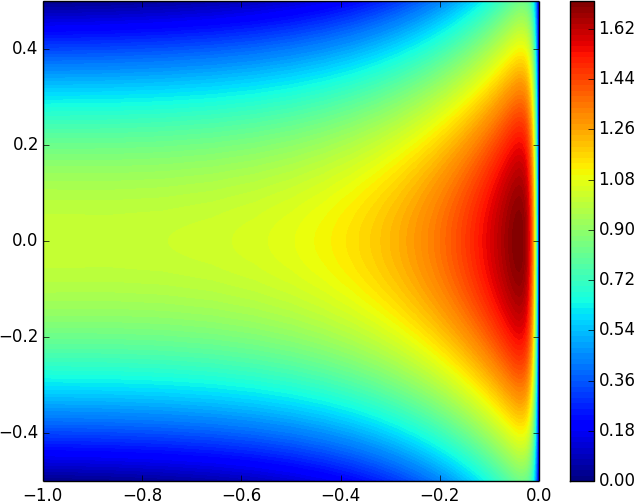
\includegraphics[width=\textwidth]{Confusion/Robustness/2d_problem_t_=_00.png}
\caption{$t=0.0$}
\end{subfigure}
\begin{subfigure}[t]{0.32\textwidth}
\centering
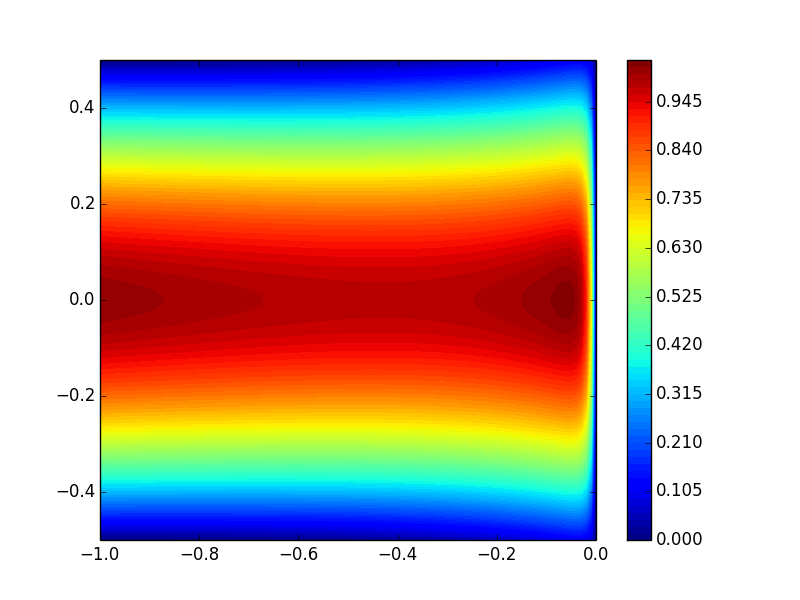
\includegraphics[width=\textwidth]{Confusion/Robustness/2d_problem_t_=_05.png}
\caption{$t=0.5$}
\end{subfigure}
\begin{subfigure}[t]{0.32\textwidth}
\centering
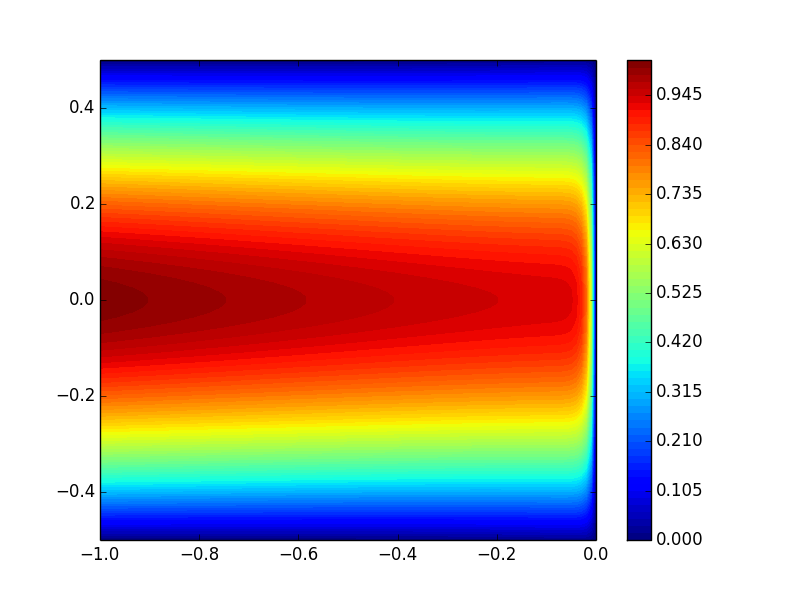
\includegraphics[width=\textwidth]{Confusion/Robustness/2d_problem_t_=_10.png}
\caption{$t=1.0$}
\end{subfigure}
\caption{Transient Eriksson-Johnson solution}
\label{fig:transientAnalytical}
\end{figure}

We provide surface plots of temporal slices of the solution at $t=0.2$ for the two norms with $\epsilon=10^{-2}$, 
and $p=2$ after 4 adaptive refinements.
The results conform to our previous experience with steady convection-diffusion where the coupled robust norm 
tends to produce smoother results in regions with sharp gradients.

\begin{figure}[ht]
\centering
\begin{subfigure}[t]{0.48\textwidth}
\centering
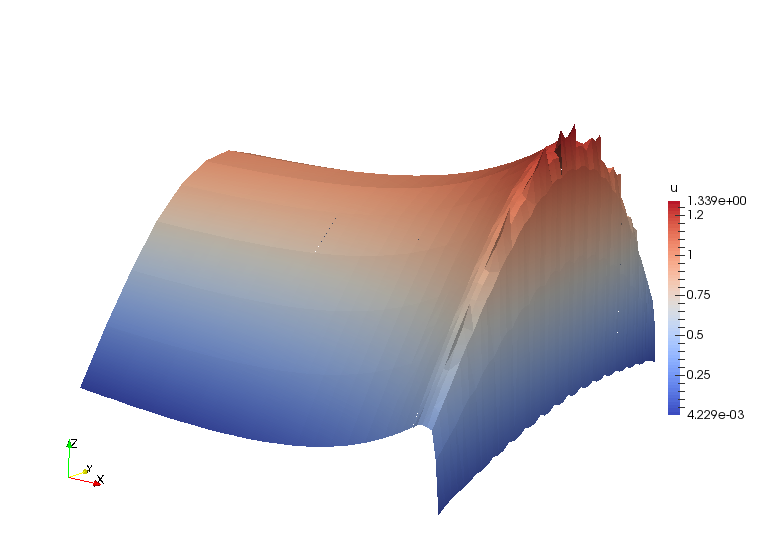
\includegraphics[width=\textwidth]{Confusion/Robustness/TransientConfusion2D_Robust_1e=2_p2_t02.png}
\caption{Robust norm}
\end{subfigure}
\begin{subfigure}[t]{0.48\textwidth}
\centering
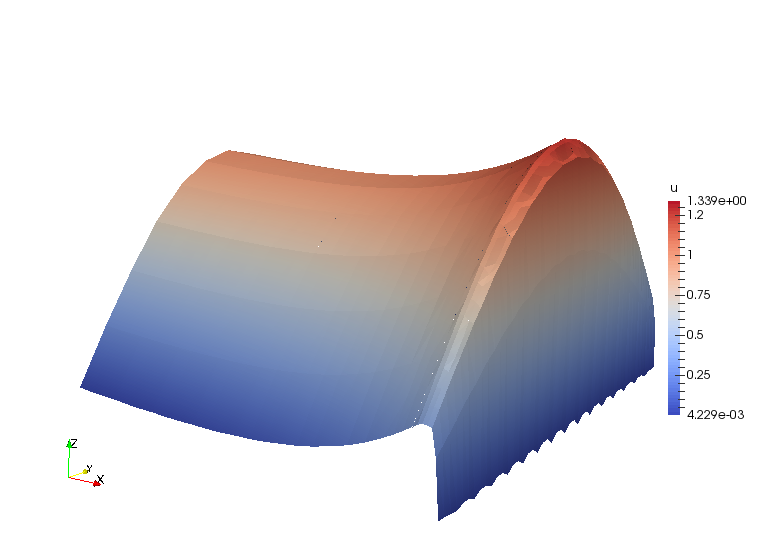
\includegraphics[width=\textwidth]{Confusion/Robustness/TransientConfusion2D_CoupledRobust_1e=2_p2_t02.png}
\caption{Coupled robust norm}
\end{subfigure}
\caption{$u$ at $t=0.2$ for $\epsilon=10^{-2}$ and $p=2$ after 4 adaptive refinements}
\label{fig:surfacePlots}
\end{figure}

% In addition to showing that the norm derived above is robust, we compare to another norm we stumbled on when working with transient compressible Navier-Stokes,
% hereafter referred to as the NS Decoupled Norm or ``NSDecoupledH1'' in the figures:
% \[
% \norm{(v,\bftau)}^2=
% \norm{\tilde\bfbeta\cdot\Gradxt v}^2
% +\norm{\Div\bftau}^2
% +\frac{1}{h^2}\norm{\bftau}^2
% +\norm{\Grad v}^2
% +\norm{v}^2\,.
% \]
% We don't have a corresponding mathematical analysis for this norm, but it appears to behave very well in every numerical test we've applied it to.

\begin{figure}[ht]
\centering
\begin{subfigure}[t]{0.45\textwidth}
\centering
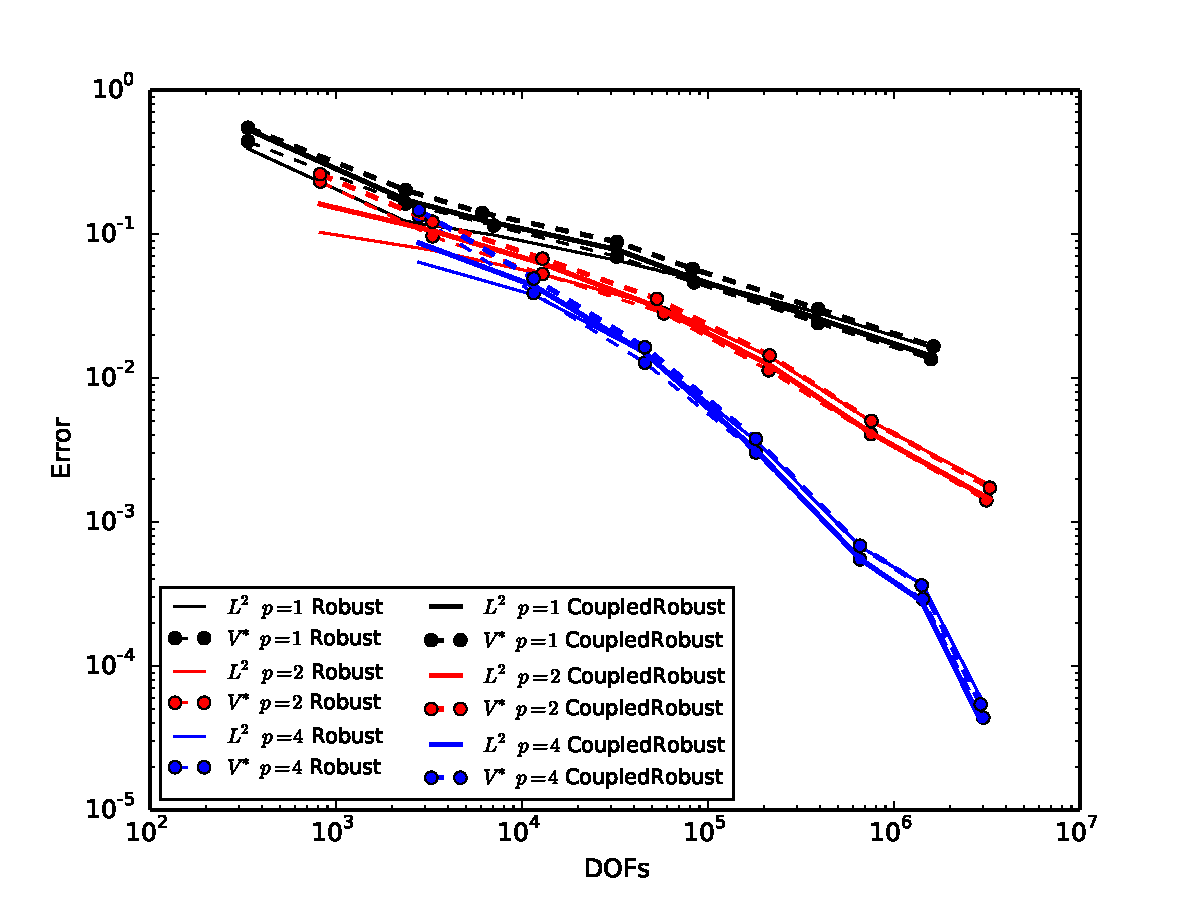
\includegraphics[width=\textwidth]{Confusion/Robustness/convergence_epsilon=1e-2.pdf}
\caption{$\epsilon=10^{-2}$}
\end{subfigure}
\begin{subfigure}[t]{0.45\textwidth}
\centering
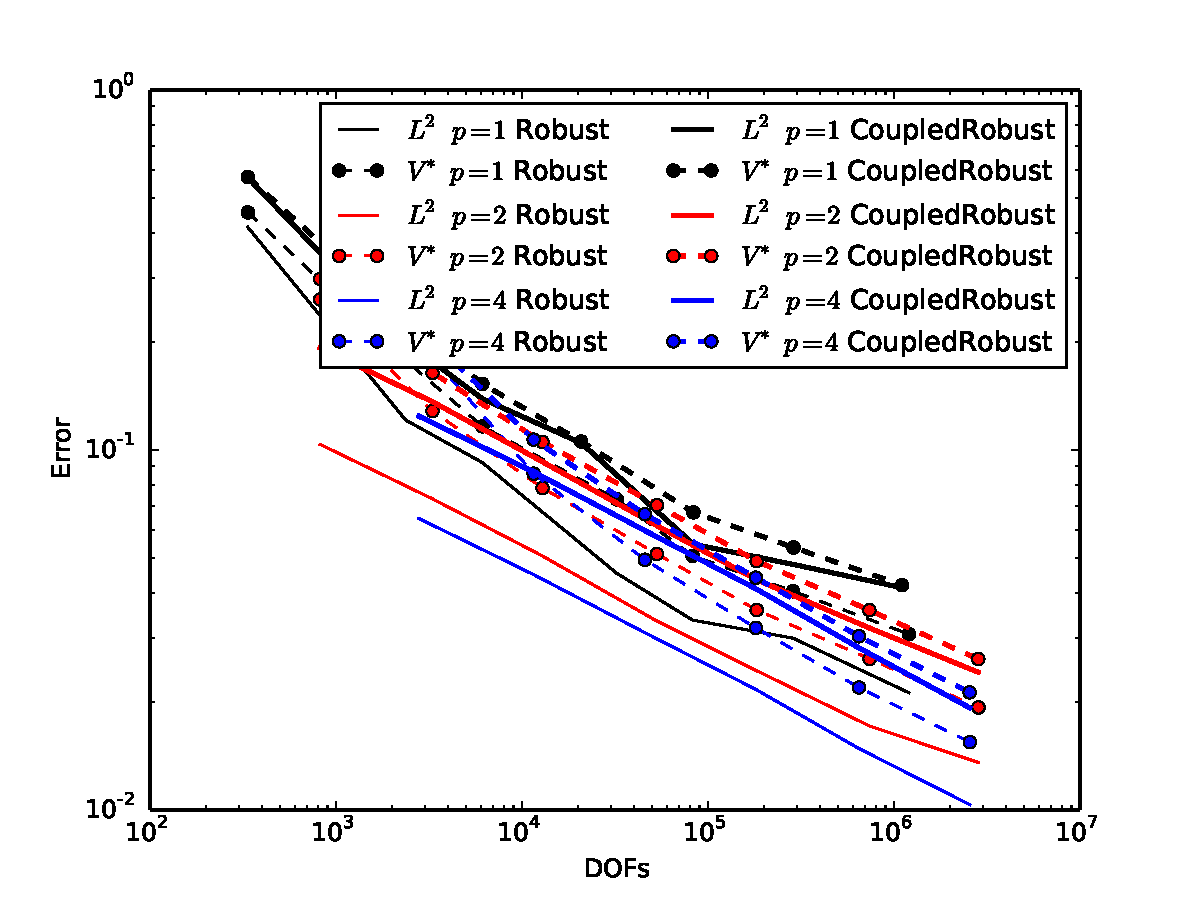
\includegraphics[width=\textwidth]{Confusion/Robustness/convergence_epsilon=1e-4.pdf}
\caption{$\epsilon=10^{-4}$}
\end{subfigure}
\begin{subfigure}[t]{0.45\textwidth}
\centering
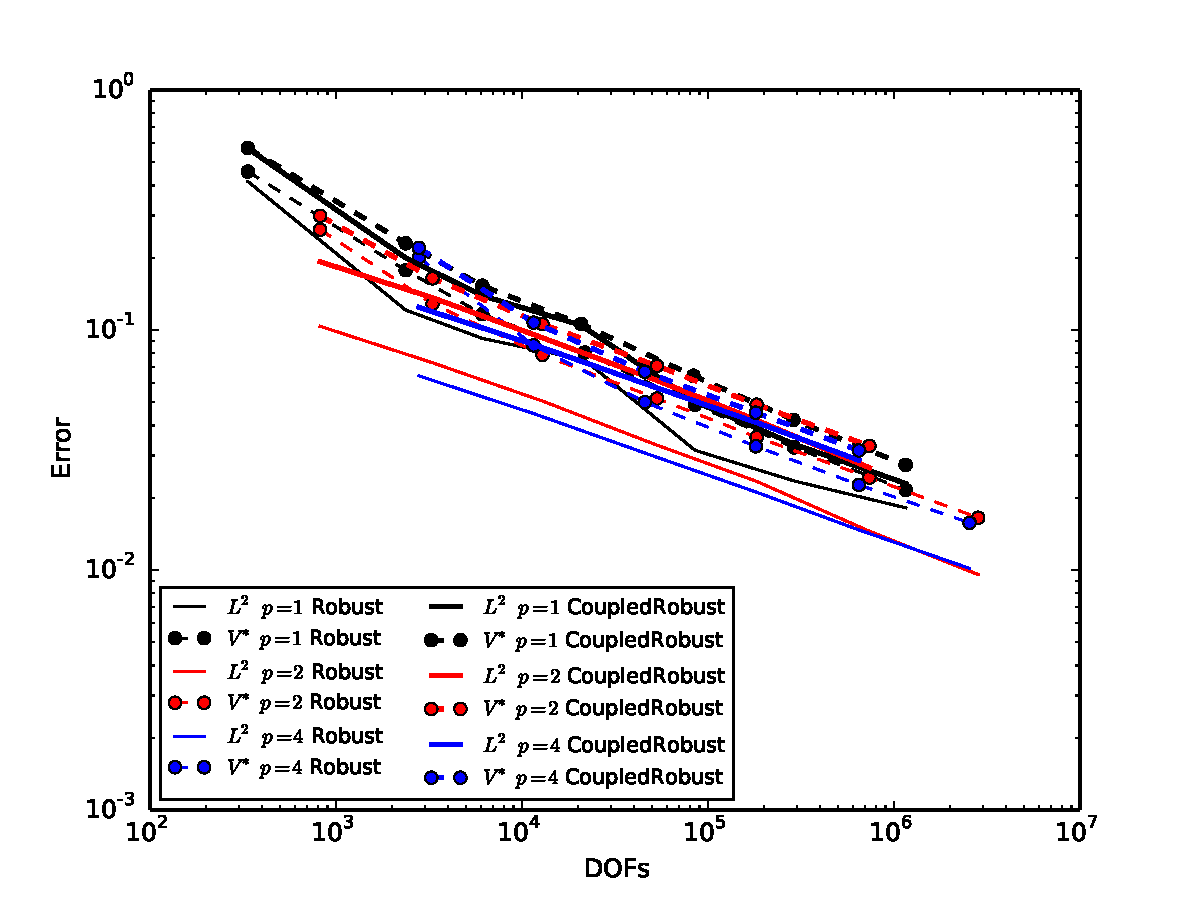
\includegraphics[width=\textwidth]{Confusion/Robustness/convergence_epsilon=1e-6.pdf}
\caption{$\epsilon=10^{-6}$}
\end{subfigure}
\begin{subfigure}[t]{0.45\textwidth}
\centering
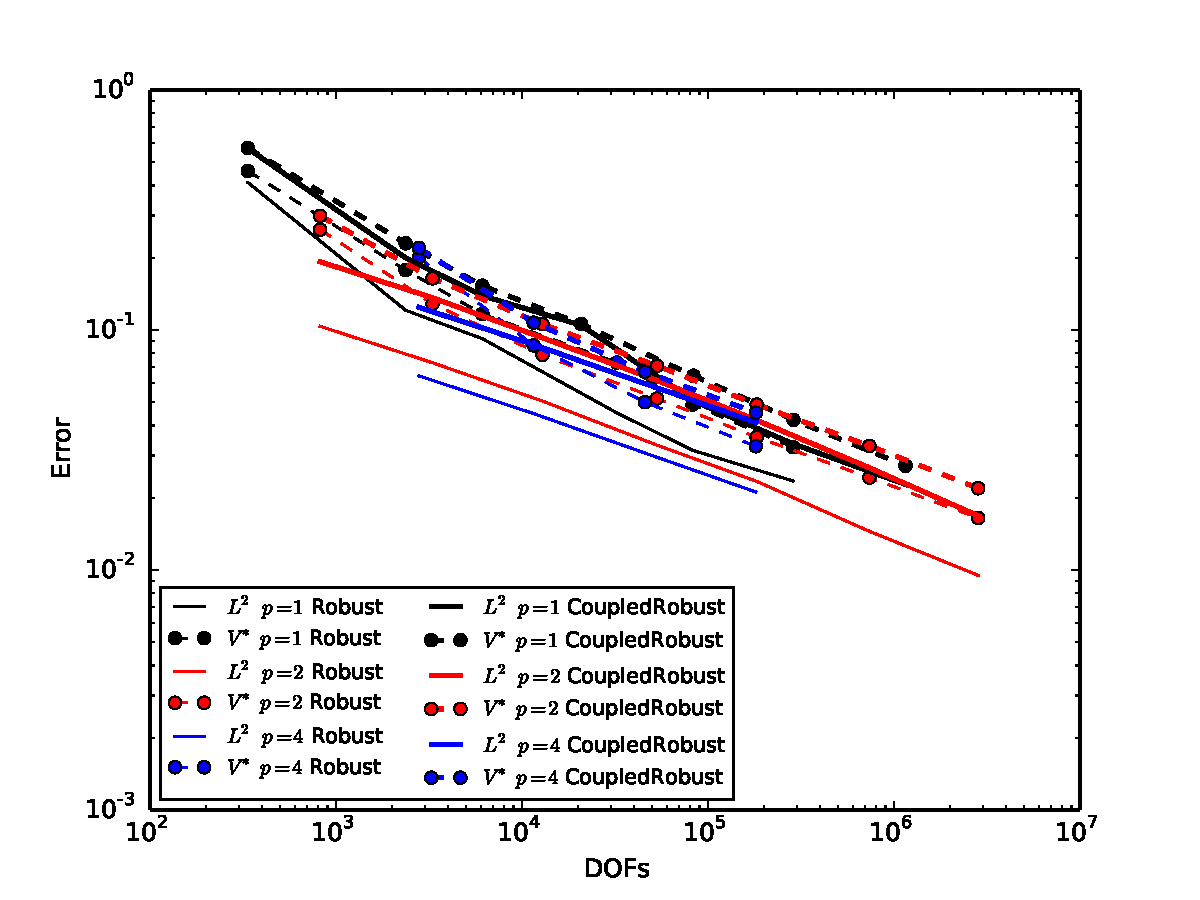
\includegraphics[width=\textwidth]{Confusion/Robustness/convergence_epsilon=1e-8.pdf}
\caption{$\epsilon=10^{-8}$}
\end{subfigure}
\caption{Convergence to analytical solution}
\label{fig:robustConvergence}
\end{figure}

\section{Summary}
As expected, convergence of the energy error appears to be a reliable predictor of convergence of the $L^2$ error. 
This relation is especially tight for moderate values of $\epsilon$. 
We've developed two robust test norms for transient convection-diffusion, though neither one guarantees robust control over $\bfsigma$ as we had
with their steady analogs. 

% \bibliographystyle{plain}  % Here the bibliography 		     %
% \bibliography{../Papers}        % is inserted.			     %
\end{document}
